\chapter{Firmware Design}
This chapter describes the firmware design principles adopted for WattMate. The implementation was mainly driven by the following objectives:

\begin{itemize}
	\item \textbf{Energy efficiency.}
	Since WattMate is intended to operate as a battery-powered embedded device, the firmware avoids unnecessary activity whenever the current system state does not require it.
	
	\item \textbf{Reliable measurement acquisition.}
	Electrical and temperature measurements are sampled at the required rate, processed consistently, and made available to the rest of the system while avoiding unnecessary latency, stale data and loss of information.
	
	\item \textbf{Responsive user interaction.}
	The local display reflects the current device state, while user inputs and BLE interactions are handled with sufficiently low latency to provide predictable behavior during normal operation.
\end{itemize}


\section{Architecture Overview}

The WattMate firmware is organized into three main layers: \texttt{device drivers}, \texttt{application tasks} and \texttt{RTOS kernel}.

\texttt{Device drivers} provide the interface between the application code and the hardware resources of the system. These resources include both internal MCU peripherals and external devices, such as the SSD1306 OLED display controller and the PAC1951 voltage/current sensor. The purpose of the drivers is to expose a simple and consistent API to the application layer, hiding the low-level hardware operations required to configure and access each peripheral.

The \texttt{application code} implements the main functionalities of WattMate by using the APIs exposed by the drivers. It is divided into multiple threads, referred to in this report as \texttt{tasks}, each responsible for a specific part of the system. Tasks communicate with each other through application events, delivered using the RTOS mechanisms of \textit{Mailboxes}. This approach avoids direct blocking calls between modules of the application code and keeps each task responsible for its own internal state. It also improves modularity, since each subsystem can be developed and maintained with limited dependencies on the others.

The task-based structure allows the RTOS to schedule the different firmware activities according to their priority and timing requirements. This is especially important for time-sensitive operations, such as BLE communication and periodic sensor acquisition. Each task is designed to avoid busy-waiting: when no operation has to be performed, the task sleeps until specific wake-up conditions instead of executing polling loops. This allows the RTOS to schedule the system efficiently and enables the power management policy to enter low-power modes whenever possible.

\begin{table}[H]
	\centering
	\caption{Overview of the main firmware levels.}
	\label{tab:firmware_levels}
	\begin{tabular}{lll}
		\toprule
		\textbf{Level} & \textbf{Role} & \textbf{Examples} \\
		\midrule
		Drivers & Hardware abstraction & PAC1951 driver, SSD1306 driver, ... \\
		App. Tasks & System functionality & Acquisition, Display, BLE, Flash, ... \\
		RTOS & Scheduling and Synchronization & Mailboxes, Sleep management, ... \\
		\bottomrule
	\end{tabular}
\end{table}

\paragraph{Original and external firmware components}
The \texttt{RTOS kernel} and the low-level MCU peripheral drivers are provided by Texas Instruments and were not modified. They were only respectively configured through the \texttt{.cfg} configuration file and the board support file (\texttt{startup/board.h}). The original code developed for this project mainly consists of the application tasks, the BLE data handling logic, the Flash storage logic, and the PAC1951 driver, for which no open-source C driver was found. The SSD1306 display driver was adapted from existing open-source C implementations and extended with project-specific APIs.

For this reason, the following sections focus mainly on the original firmware components developed for WattMate. External or vendor-provided code is discussed only when its behavior is relevant to explain a specific design choice.

\section{Application Tasks}

The application-level tasks used to implement the WattMate firmware are located mainly in 
\texttt{WattMate\_BLE/Startup/Tasks} and \texttt{WattMate\_BLE/Application}. 
They are listed below:

\begin{itemize}
	\item \textbf{App:}
	This is the main application task. It maintains and updates the global state of the device by processing events received from the other tasks and coordinating the behavior of the different subsystems according to runtime policies. In general, the App task does not handle low-level hardware details directly; instead, it sends high-level requests to the other tasks, which are responsible for executing them in the appropriate timing and hardware context.
	
	\item \textbf{Display:}
	This task handles the OLED Display user interface. It receives commands from the App task, which controls the general display state. The Display task stores the layout of each visible page, manages screen updates, animations and standby timing, and exclusively owns the SSD1306 driver handling.
	
	\item \textbf{Flash Storage:}
	This task manages persistent firmware-produced data stored in the internal Flash memory. It exposes APIs to store and retrieve the data records, while hiding the details of Flash page organization, record placement, writing, validation, and erase handling from the rest of the application.
	
	\item \textbf{Input:}
	This task manages inputs that are handled by internal MCU peripherals. It handles the user button, including debounce and long-press detection, and controls the ADC sampling and NTC Enable output GPIO used to read the NTC temperature sensor. The App task is notified only when a relevant input event or a new temperature sample is available, avoiding continuous polling.
	
	\item \textbf{PAC:}
	This task manages the acquisition flow of the PAC1951 sensor. It receives high-level requests from the App task and configures the timing and sensor settings according to predefined sampling profiles. When a new electrical measurement is obtained from the PAC1951 driver, the App task is notified through an event, avoiding continuous polling.
	
	\item \textbf{WattMate BLE:}
	This task manages the BLE interface of WattMate. It handles advertising, connection state changes, the custom GATT service, telemetry notifications, and control/configuration commands received from the mobile application. BLE events that affect the device behavior are translated into application events and forwarded to the App task.
	
	
\end{itemize}

\subsection{Task Communication Model}

Communication between firmware tasks is mainly based on event messages. When a task, a timer callback, or an interrupt callback needs to notify another part of the system, it posts an event message into the mailbox of the destination task. The receiving task sleeps while no message is pending on its mailbox, so no busy-waiting loop is required. Once a pending message arrives in the mailbox of a task, the task is woken up according to its priority assigned in the RTOS scheduler, and the required operations can be performed.

\begin{figure}[H]
	\centering
	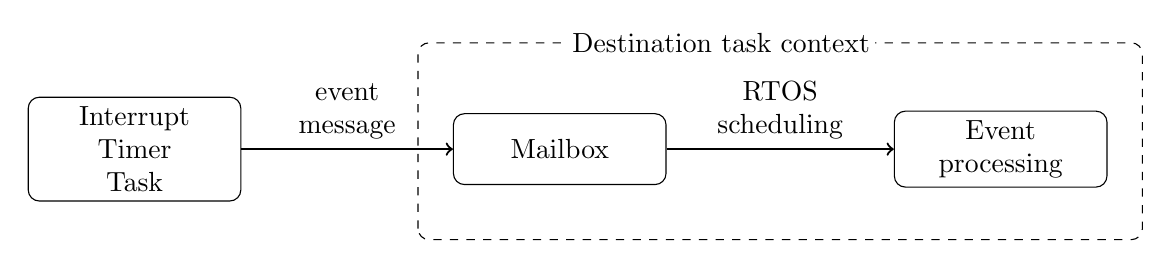
\begin{tikzpicture}[
		block/.style={
			draw,
			rounded corners,
			align=center,
			minimum height=0.9cm,
			minimum width=2.7cm
		},
		context/.style={
			draw,
			rounded corners,
			dashed
		},
		arrow/.style={->, thick}
		]
		
		```
		% Blocks
		\node[block] at (0,0) (source) {Interrupt\\Timer\\Task};
		\node[block] at (5.4,0) (mailbox) {Mailbox};
		\node[block] at (11,0) (processing) {Event\\processing};
		
		% Destination task context
		\draw[context] (3.6,-1.15) rectangle (12.8,1.35);
		\node[fill=white, inner sep=2pt] at (7.45,1.35) {Destination task context};
		
		% Arrows
		\draw[arrow] (source.east) -- node[above, align=center] {event\\message} (mailbox.west);
		\draw[arrow] (mailbox.east) -- node[above, align=center] {RTOS\\scheduling} (processing.west);
		
	\end{tikzpicture}
	\caption{Event-based communication model between firmware tasks.}
	\label{fig:task_communication_model}
	
\end{figure}

This model avoids busy-waiting loops and reduces direct dependencies between modules. Interrupt and timer callbacks are kept short, since they only post the corresponding event message, while the actual processing is deferred to the destination task context.

\subsection{Task Scheduling and Priorities}

The event-based communication model only defines how tasks are notified. The actual execution order of tasks that simultaneously require CPU time is still controlled by the TI-RTOS scheduler. In practice, when a message is posted to the mailbox of a blocked task, that task becomes ready to execute, but this does not necessarily mean that it immediately receives CPU time. The scheduler selects which ready task is executed according to the configured scheduling policy~\cite{ti_sysbios_user_guide}, based on task priorities.


This behavior is exploited in the firmware design to separate tasks with different characteristics, with the final goal of guaranteeing the correct behavior of the whole system, from the time-sensitive functionalities to the ones that can handle a longer latency. The idea is that the system must remain responsive to external inputs, while the internal computations can wait for the CPU to be available before being performed.

The resulting priority assignment is summarized in Table~\ref{tab:task_priorities}. In TI-RTOS, task priorities are numeric and increase with the assigned value; therefore, a task with priority 3 has higher priority than a task with priority 2 or 1~\cite{ti_sysbios_task}.

\begin{table}[H]
	\centering
	\small
	\setlength{\tabcolsep}{4pt}
	\renewcommand{\arraystretch}{1.25}
	\caption{Firmware task priority assignment.}
	\label{tab:task_priorities}
	\begin{tabularx}{\textwidth}{
			@{}
			>{\raggedright\arraybackslash}p{2.3cm}
			>{\centering\arraybackslash}p{1.5cm}
			>{\raggedright\arraybackslash}X
			@{}
		}
		\toprule
		\textbf{Task} &
		\textbf{Priority} &
		\textbf{Design rationale}
		\tabularnewline
		\midrule
		
		BLE & 3 &
		Must remain as responsive as possible in order to satisfy the strict time constraints of the BLE protocol, maintain the connection, and exchange data with the mobile application.
		\tabularnewline
		
		PAC & 2 &
		Electrical measurements are part of the core monitoring function and should be handled with limited latency.
		\tabularnewline
		
		Input &	2 &
		User input should be processed quickly enough to make the device feel responsive. In addition, the ALERT input from the PAC1951 should be handled as quickly as possible, in order to respond quickly to dangerous situations.
		\tabularnewline
		
		App & 1 &
		Coordinates the main application logic, but it does not contain time-sensitive handling.
		\tabularnewline
		
		Flash Storage & 1 &
		Flash operations are marginal from the point of view of pure functionality, and can therefore tolerate latency if necessary.
		\tabularnewline
		
		Display & 1 &
		Display updates are human-facing operations and can tolerate small delays without being noticed by the user.
		\tabularnewline
		\bottomrule
	\end{tabularx}
	
\end{table}

The priority assignment therefore defines the practical behavior of the event-driven architecture. A low-priority task can be woken up by a message and still wait before running if higher-priority tasks are ready at the same time. As a result, heavier computations, such as SoC and SoH estimation, can coexist with time-sensitive activities, such as BLE handling, without introducing direct blocking effects or noticeable misbehaviors.

It is important to note that the scheduler is not modified by the project, and the stock TI-RTOS one is used; only the task priorities and the event-based execution structure are configured to match the firmware requirements.


\subsection{Main Application Task}
\label{Main_Application_Task}

The App task is the central coordination point of the WattMate firmware. Its main role is to maintain the global application state and to decide how the other subsystems should behave according to the current operating condition. For this reason, it receives events from the PAC, Input, Display, Flash Storage and BLE tasks, updates its internal state, and sends high-level requests back to the appropriate subsystem when an action is required.

\paragraph{Runtime resource policy.}
One of the main responsibilities of the App task is handle all the resources avaiable, in order to reduce as much as possible the power consumption. The firmware does not keep all measurements and data streams permanently active. In particular the following policies are applied:
\begin{itemize}
	\item \textbf{PAC1951 sampling profile.}
	The PAC1951 sampling profile controls the internal behavior of the sensor itself, independently from whether the MCU is currently reading data from it through I2C. The App task requests the PAC1951 \texttt{normal profile} only when electrical activity is present on the power bus; otherwise, it requests the \texttt{idle profile}.
	
	It is important to note that the \texttt{idle profile} is not simply a deep-sleep mode for the PAC1951. Even in this state, the sensor remains configured to monitor the battery line and to generate an alert when relevant electrical activity is detected again. This alert mechanism is necessary because the MCU does not always read the PAC1951 continuously through I2C; therefore, when I2C communication is suspended, the MCU has no direct information about the current state of the power bus. The PAC1951 alert pin provides a notification that the bus has become active again, allowing the firmware to wake up the corresponding logic, re-evaluate the system state, and request the PAC1951 \texttt{normal profile} if when needed. More details about the two PAC profiles are provided in Section~\ref{PAC_Application_Task}.
	
	
	\item \textbf{PAC1951 measurement stream.}
	The measurement stream controls the I2C communication between the MCU and the PAC1951. When the stream is enabled, the PAC task periodically reads the latest electrical measurements from the sensor through the I2C bus and forwards updated snapshots to the App task. When the stream is disabled, the PAC1951 can still keep its configured sampling profile, but the MCU avoids periodic I2C transactions.
	
	The stream is enabled only when live electrical measuremet data are needed by the rest of the system, such as when the display is on, or when the BLE application is requesting telemetry. If none of these conditions is true, the stream is released, allowing the MCU to remain in sleep mode for longer periods and helping the RTOS power policy enter deep low-power states.
	
	\item \textbf{Temperature ADC sampling.}
	Similarly to the Electrical PAC1951 measures, the NTC temperature measurement is also managed as an on-demand resource. The ADC sampling is enabled in the Input Task only when temperature information is needed, for example when the display is currently showing a page that requires temperature data, or when the BLE application is requesting live telemetry. This allows the MCU to remain in sleep mode for longer periods and helps the RTOS power policy enter deep low-power states.
	
	\item \textbf{Energy accumulation.}
	PAC1951 energy accumulation I2C reading, performed by the PAC Task, is enabled only when the accumulated energy is useful for the current firmware state, for example when the display or BLE interface requires energy-related information. Separating live electrical measurements from energy accumulation allows the firmware to avoid unnecessary I2C communications.
	
	\item \textbf{Display dimming and standby.}
	The OLED display is not kept fully active permanently. After a period without user interaction (\SI{20}{s}), the App task requests a low-luminosity state for the display. If the inactivity continues for an additional \SI{10}{s}, the display is turned off. A user button press wakes up the display again.
	
	This policy reduces the system power consumption in both a direct and an indirect way. Directly, dimming or turning off the display lowers the energy required by the OLED itself. Indirectly, the display state also influences the rest of the runtime policy: when the display is completely off, live measurement streams are kept active only if they are still required by another subsystem, such as the BLE application. In this way, the firmware avoids keeping acquisition and update activity enabled only for a user interface that is not currently visible.
	
	
	
	\item \textbf{BLE advertising.}
	BLE advertising is enabled only when the device must be discoverable, therefore when no active BLE connection is open. The advertising frequency is also dynamically changed by the firmware: fast advertising (\SI{100}{ms} period) is used for a limited time (\SI{20}{s} period) at startup and after a user button press, while slow advertising (\SI{1}{s} period) is used in the remaining conditions. This keeps the device available for connection, although with longer discovery times, while reducing the power consumption associated with BLE when the user is not actively interacting with WattMate.
	
	\item \textbf{BLE data stream.}
	BLE telemetry streaming is enabled only when requested by the mobile application. This prevents the firmware from continuously preparing and sending BLE notifications when no client is actively using live data.
	
	\item \textbf{BLE connection supervision.}
	The BLE connection is kept active as long as the central device remains reachable. The firmware does not require a continuous application-level data exchange to maintain the connection; this is handled by the BLE link layer. However, if the phone becomes unreachable, for example because it is turned off or moved out of range, the connection eventually expires through the BLE supervision timeout (\SI{2}{s}). In that case, the firmware processes the disconnection event and returns WattMate to the advertising state, instead of remaining associated with a non-responsive device.
	
\end{itemize}

\paragraph{Measurement freshness.}
Considering the Resource Policies, it is clear that the App task has no guarantee to receive a constant stream measured data at all times. Because of this, App task keeps track of the validity of the latest measurements. Electrical, energy, and temperature data are marked as fresh only for a limited time after a new sample is received. If no updated sample arrives before the corresponding timeout expires, the data are marked as not fresh, preventing the display, BLE telemetry, and battery estimation logic from using outdated values as if they were current measurements.

\begin{table}[H]
	\centering
	\small
	\caption{Measurement data freshness timeouts}
	\label{tab:data_freshness}
	\begin{tabular}{ll}
		\toprule
		\textbf{Measurement Type} & \textbf{Timeout} \\
		\midrule
		PAC Live Data  & 500 ms  \\
		PAC Energy     & 500 ms  \\
		Temperature    & 2000 ms \\
		\bottomrule
	\end{tabular}
\end{table}

\paragraph{Battery operating conditons.}
The App task is responsible for estimating the battery-related statistics used by WattMate. The firmware first reconstructs the operating condition of the battery by detecting charge and discharge sessions from the PAC1951 measurements. The same data are then processed to update energy, State of Charge, State of Health, and cycle-related information.

A session is detected from the instantaneous power measured on the power bus. The firmware compares the measured power with predefined start and stop thresholds to determine whether the battery is being charged (state \texttt{CHARGE}), discharged (state \texttt{DISCHARGE}), or if no active session is present (state \texttt{IDLE}). The use of separate start and stop thresholds introduces hysteresis, preventing unstable transitions caused by small power fluctuations around zero.

When the measured power falls below the corresponding stop threshold, the session is moved to \texttt{PAUSED} instead of being immediately closed. The session is terminated only if the inactive condition persists until the timeout expires, allowing short interruptions to be tolerated without splitting a single physical charge or discharge process into multiple independent sessions.

This behavior is summarized by the finite-state machine shown in Figure~\ref{fig:session_fsm}.

\begin{figure}[H]
	\centering
	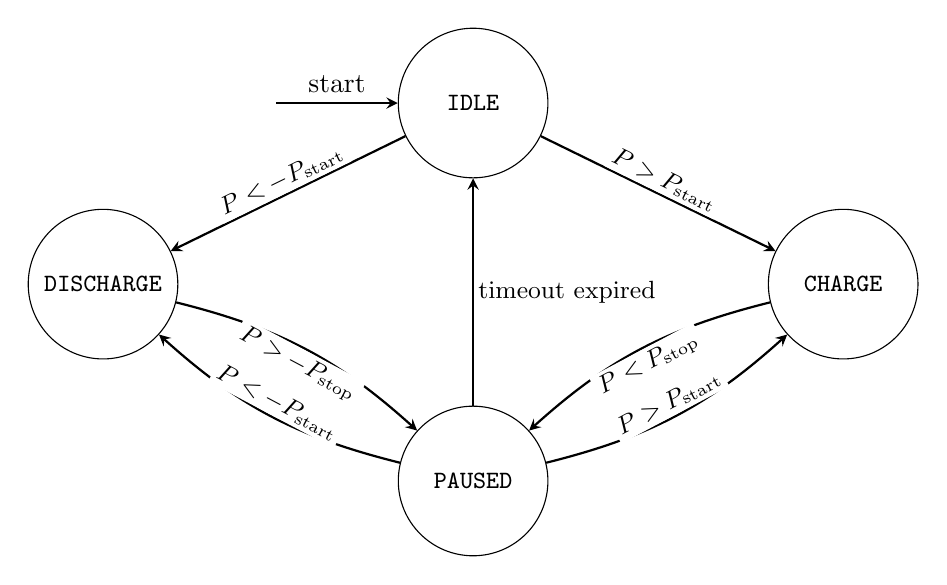
\begin{tikzpicture}[
		>=stealth,
		state/.style={
			draw,
			circle,
			minimum size=1.9cm,
			inner sep=1pt,
			align=center,
			font=\small\ttfamily
		},
		trans/.style={->, thick},
		lab/.style={
			font=\small,
			fill=white,
			inner sep=1.5pt
		}
		]
		
		% States
		\node[state] (idle) at (0,3.0) {IDLE};
		\node[state] (charge) at (4.7,0.7) {CHARGE};
		\node[state] (discharge) at (-4.7,0.7) {DISCHARGE};
		\node[state] (paused) at (0,-1.8) {PAUSED};
		
		% Initial arrow
		\draw[trans] (-2.5,3.0) -- node[above] {start} (idle.west);
		
		% Session start
		\draw[trans] (idle) -- node[lab, above, sloped] {$P > P_{\mathrm{start}}$} (charge);
		\draw[trans] (idle) -- node[lab, above, sloped] {$P < -P_{\mathrm{start}}$} (discharge);
		
		% Charge pause / resume
		\draw[trans] (charge) to[bend right=14]
		node[lab, below, sloped] {$P < P_{\mathrm{stop}}$}
		(paused);
		
		\draw[trans] (paused) to[bend right=14]
		node[lab, above, sloped] {$P > P_{\mathrm{start}}$}
		(charge);
		
		% Discharge pause / resume
		\draw[trans] (discharge) to[bend left=14]
		node[lab, below, sloped] {$P > -P_{\mathrm{stop}}$}
		(paused);
		
		\draw[trans] (paused) to[bend left=14]
		node[lab, above, sloped] {$P < -P_{\mathrm{start}}$}
		(discharge);
		
		% Session termination
		\draw[trans] (paused) -- node[lab, right] {timeout expired} (idle);
		
	\end{tikzpicture}
	\caption{Finite-state machine used for session detection from the measured power.}
	\label{fig:session_fsm}
\end{figure}

\paragraph{Battery statistics estimation.}
Once a charge or discharge session has been identified, the App task uses the
session information to compute higher-level battery statistics. These quantities
are derived from the energy exchanged during detected sessions, rather than from
instantaneous voltage or current values alone.

The estimation method is based on energy integration at the USB bus. This gives
a reliable measurement of the energy that entered or left the system during a
session, but it does not directly reveal the absolute battery State of Charge.
WattMate is placed on the USB power path and does not directly observe the
battery cell voltage or the electrochemical end-of-charge/end-of-discharge
conditions. Therefore, SoC and SoH estimation require explicit operating
assumptions.

The firmware assumes that a completed charge or discharge session corresponds to
a known battery endpoint:
\[
\begin{cases}
	\texttt{CHARGE completed} & \Rightarrow \mathrm{SoC} = 100\% \\
	\texttt{DISCHARGE completed} & \Rightarrow \mathrm{SoC} = 0\%
\end{cases}
\]
This assumption provides the absolute reference point that energy integration
alone cannot provide. Before the first completed session, the SoC is therefore
marked as \texttt{UNKNOWN}. After the first completed session, the SoC is set to either 0\% or 100\%, depending on the direction of the session, and the eitimation of SoC can atually begin.

During an active session, the firmware computes the energy exchanged since the
session started, denoted as \(E_{\mathrm{session}}\). This value is compared with
the best available estimate of the usable battery energy:
\[
\mathrm{progress} =
\frac{E_{\mathrm{session}}}{E_{\mathrm{usable}}} \cdot 100
\]
The SoC is then obtained according to the session direction:
\[
\mathrm{SoC} =
\begin{cases}
	\mathrm{progress} & \text{during charge} \\
	100 - \mathrm{progress} & \text{during discharge}
\end{cases}
\]

Before a measured usable-energy reference is available, the firmware can only use
the nominal battery energy configured through BLE. In this case, the SoC is
reported as \texttt{ESTIMATED}. Once at least one completed sessions have been observed, the energy measured during a completed endpoint-to-endpoint session can be used as the usable-energy reference, and the SoC estimate can be promoted to \texttt{LEARNED}.

The \textit{State of Health} is computed by comparing the measured usable energy
with the nominal battery energy:
\[
\mathrm{SoH} =
\frac{E_{\mathrm{usable}}}{E_{\mathrm{nominal}}} \cdot 100
\]
This estimate is meaningful only if the completed session used as reference is
representative of a full usable-capacity interval. In other words, the operating
assumption is that completed charge and discharge sessions reach the actual
battery endpoints. If a session is interrupted before the battery reaches the
corresponding endpoint, the measured energy no longer represents the full usable
capacity and the SoH estimate may be biased.

The maturity of the estimates is summarized in
Table~\ref{tab:battery_estimation_maturity}.



\begin{table}[H]
	\centering
	\small
	\setlength{\tabcolsep}{4pt}
	\renewcommand{\arraystretch}{1.5}
	\caption{Battery estimation maturity during firmware operation.}
	\label{tab:battery_estimation_maturity}
	\begin{tabularx}{\textwidth}{
			@{}
			>{\raggedright\arraybackslash}p{3.0cm}
			>{\raggedright\arraybackslash}X
			>{\raggedright\arraybackslash}p{3.5cm}
			>{\raggedright\arraybackslash}p{3.5cm}
			@{}
		}
		\toprule
		\textbf{Stage} &
		\textbf{Available information} &
		\textbf{SoC status} &
		\textbf{SoH status} \\
		\midrule
		
		Startup / reset &
		Nominal battery energy (if configured from BLE); &
		\texttt{UNKNOWN}. Total energy yconsumed during first cycle is unknown. &
		\texttt{UNKNOWN}. No measured battery energy available. \\
		
		After first completed session &
		Nominal battery energy (if configured from BLE). A charge or discharge endpoint is assumed to have been reached. &
		\texttt{ESTIMATED}. SoC is computed using the nominal battery energy and Energy since the start of current session. &
		\texttt{UNKNOWN}. No measured battery energy available. \\
		
		After second completed sessions &
		Nominal battery energy (if configured from BLE), measured battery energy.  &
		\texttt{LEARNED}. SoC is computed using the last measured battery energy and current session energy  &
		\texttt{LEARNED}. SoH is computed using the last measured battery energy \\
		
		\bottomrule
	\end{tabularx}
\end{table}


\paragraph{Interaction with persistent storage.}
Persistent storage, handled by the Flash Storage Task, is used to keep the battery estimation state across resets and power cycles. Without this mechanism, WattMate would lose the learned battery history every time the device restarts, forcing the estimation process to start again from an unknown state.

The App task stores two different classes of data:

\begin{itemize}
	\item \textbf{Fast records.}
	These records are used as checkpoints for an active charge or discharge session. They store the current accumulated session energy and a small set of flags describing the state of the ongoing cycle. Fast records are written periodically, every \SI{30}{s}, instead of after every PAC1951 measurement. This limits the number of Flash write operations and reduces memory wear.
	
	If the device resets during an active session, the latest fast record can be used to restore an approximate session state. The restored energy is not considered \texttt{LEARNED}, and instead is set to \texttt{ESTIMATED}, because the checkpoint may be older than the last measurement acquired before the reset. Any energy exchanged between the last checkpoint and the reset is therefore not included in the restored value.
	
	For this reason, the firmware propagates an estimation-quality flag together with the energy values used for battery statistics. The rule is conservative: if at least one input of a calculation is \texttt{UNKNOWN}, the result is marked as \texttt{UNKNOWN}; otherwise, if at least one input is \texttt{ESTIMATED}, the result is marked as \texttt{ESTIMATED}; only values computed entirely from learned inputs are marked as \texttt{LEARNED}. The effect of this rule after a checkpoint restoration is summarized in Table~\ref{tab:checkpoint_quality_propagation}.
	
	
	\begin{table}[H]
		\centering
		\small
		\setlength{\tabcolsep}{4pt}
		\renewcommand{\arraystretch}{1.25}
		\caption{Quality propagation after checkpoint restoration.}
		\label{tab:checkpoint_quality_propagation}
		\begin{tabularx}{\textwidth}{
				@{}
				>{\raggedright\arraybackslash}p{3.cm}
				>{\raggedright\arraybackslash}X
				>{\raggedright\arraybackslash}p{3.5cm}
				>{\raggedright\arraybackslash}p{3.5cm}
				@{}
			}
			\toprule
			\textbf{Situation}					&
			\textbf{Effect on stored values}	&
			\textbf{SoC Quality} 				&
			\textbf{SoH Quality} 				\\
			\midrule
			
			Reset during an active session &
			The current-cycle energy is restored from the latest fast checkpoint and marked as \texttt{ESTIMATED}. & \texttt{ESTIMATED}, because current cycle energy is \texttt{ESTIMATED} &
			Not affected, because it uses last-session energy \\
			
			After the restored session completed &
			The completed-session energy is stored as the last completed-cycle energy, but with \texttt{ESTIMATED} quality &
			\texttt{ESTIMATED}. Starts from 0\% or 100\% with \texttt{LEARNED} current-cycle session energy, but it uses an \texttt{ESTIMATED} last-session energy &
			\texttt{ESTIMATED}. Because it uses an \texttt{ESTIMATED} last-session energy \\
			
			After the endpoint-to-endpoint session completed &
			The completed-cycle energy is measured and so it is marked as \texttt{LEARNED} &
			\texttt{LEARNED}, both current and last-session energy are \texttt{LEARNED} &
			\texttt{LEARNED}, last-session energy is \texttt{LEARNED}\\
			
			\bottomrule
		\end{tabularx}
	\end{table}
	
	
	\item \textbf{Slow records.}
	These records store the slower-changing battery estimation history. They include the nominal battery energy, the last completed cycle energy, the number of completed cycles, and the last completed session type. Slow records are updated when this higher-level state changes, mainly at the end of a session or when the battery configuration is modified via BLE.
	
	Slow records represent the learned battery history used by the firmware after a restart. They allow WattMate to preserve the estimation maturity reached during previous operation instead of returning to the initial unknown state.
\end{itemize}

The stored battery data can be cleared when the battery is replaced. This reset can be triggered either from the BLE interface or through a long press of the User Button, forcing the firmware to discard the previous battery history and rebuild the estimation state for the new battery.

\subsection{Display Application Task}

The Display Application task manages the local OLED user interface of WattMate. Its role is limited to the presentation layer: it defines the UI pages, display timing, brightness policy, screen update logic, and transitions between the different visual states. The task does not perform measurements and does not compute the values shown to the user.

The App task interacts with the Display task through high-level display commands posted to its TI-RTOS mailbox. These commands do not directly access the OLED driver or modify the rendered content; they only request UI-level actions. The detailed execution is handled internally by the Display task, which remains responsible for the UI state machine and for the SSD1306 display driver state machine. The main command categories are summarized in Table~\ref{tab:display_commands}.

\begin{table}[H]
	\centering
	\small
	\caption{Main command categories handled by the Display task.}
	\label{tab:display_commands}
	\begin{tabularx}{\textwidth}{lX}
		\toprule
		\textbf{Command category} & \textbf{Purpose} \\
		\midrule
		Initialization		& Start the display task and show the initial UI sequence. \\
		Page control		& Select the initial page or move to the next page. \\
		Brightness control	& Switch between normal and low-luminosity display modes. \\
		Power state control	& Turn the OLED display on or off. \\
		Refresh control		& Request an immediate redraw of the currently active page, over-riding the Display Task defined Refresh Rate. \\
		\bottomrule
	\end{tabularx}
\end{table}

\paragraph{Displayed data input.}
The values shown on the screen are not passed through the Display task mailbox. The mailbox is only used for high-level display commands, while the displayed data are obtained by reading a snapshot of the current application state produced by the App task.

This design reduces mailbox traffic and decouples the display refresh rate from the measurement acquisition rate. As a result, the Display task can autonomously manage UI timing, state transitions, and rendering, while always using the most recent application data available at redraw time.

\paragraph{Page organization}
The user interface is organized into a small set of pages. Similar information is
grouped together so that each page remains readable on the small OLED display:

\begin{itemize}
	\item \textbf{Live electrical measurements pages:} they show the
	live electrical measurements, namely voltage, current, power, and temperature, together with the maximum values reached during the current session.
	
	\begin{center}
		\captionsetup{type=figure,width=0.70\textwidth,font=small}
		
		\begin{minipage}{0.30\textwidth}
			\centering
			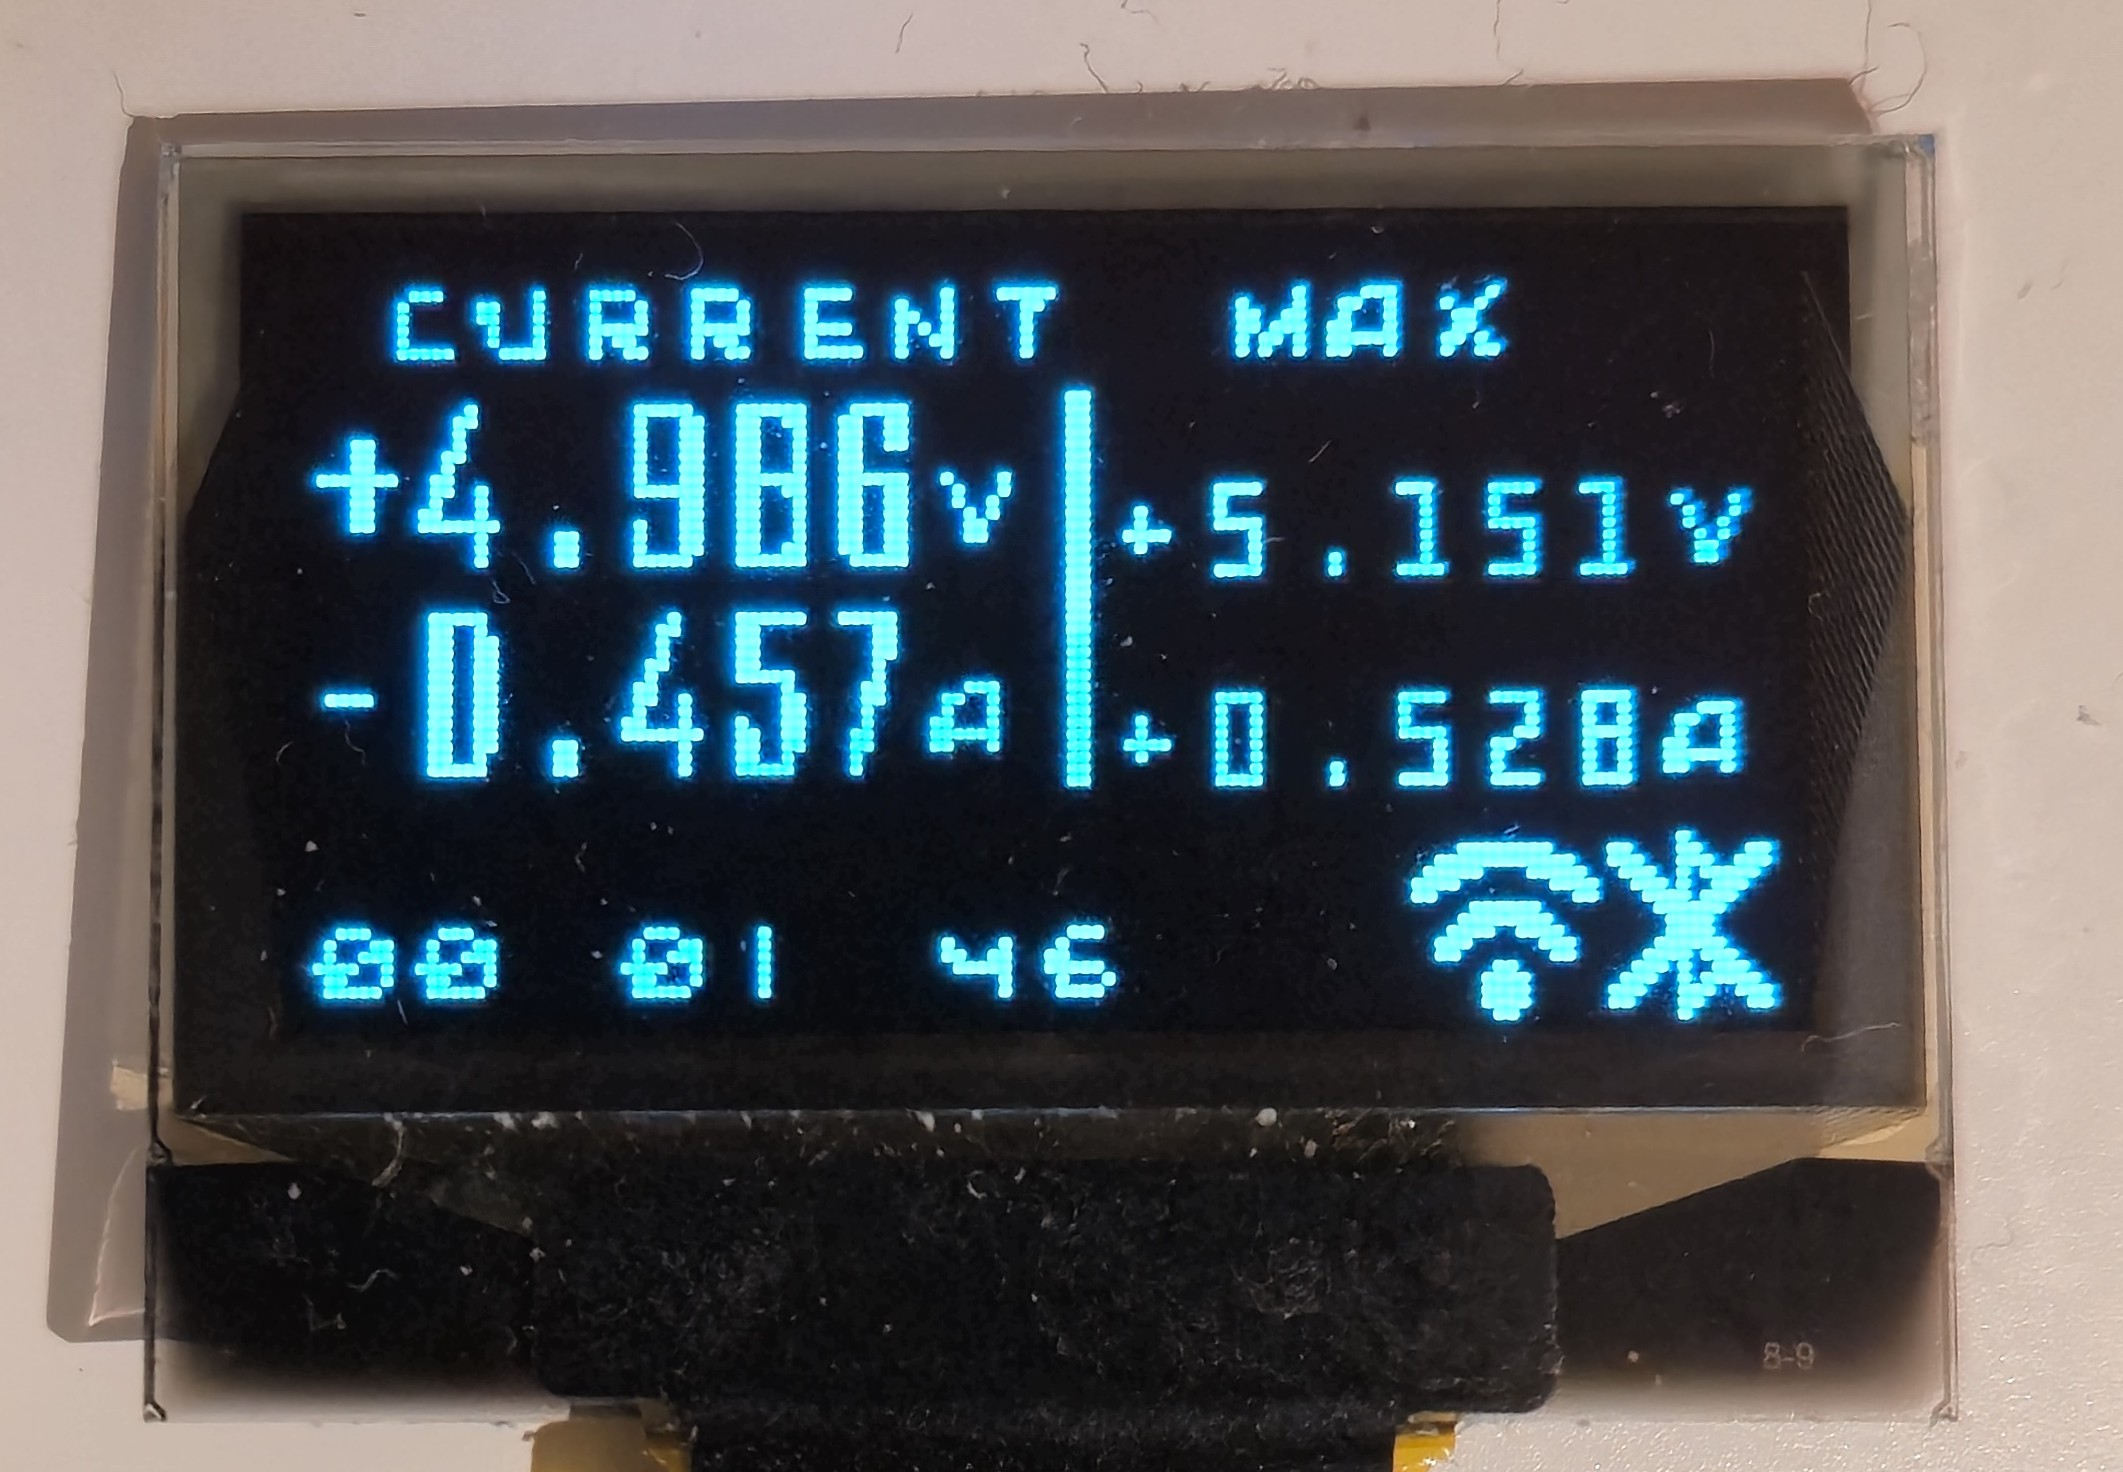
\includegraphics[width=\textwidth]{figures/3_FW_Figures/Page1.jpg}
		\end{minipage}
		\hspace{1.2cm}
		\begin{minipage}{0.30\textwidth}
			\centering
			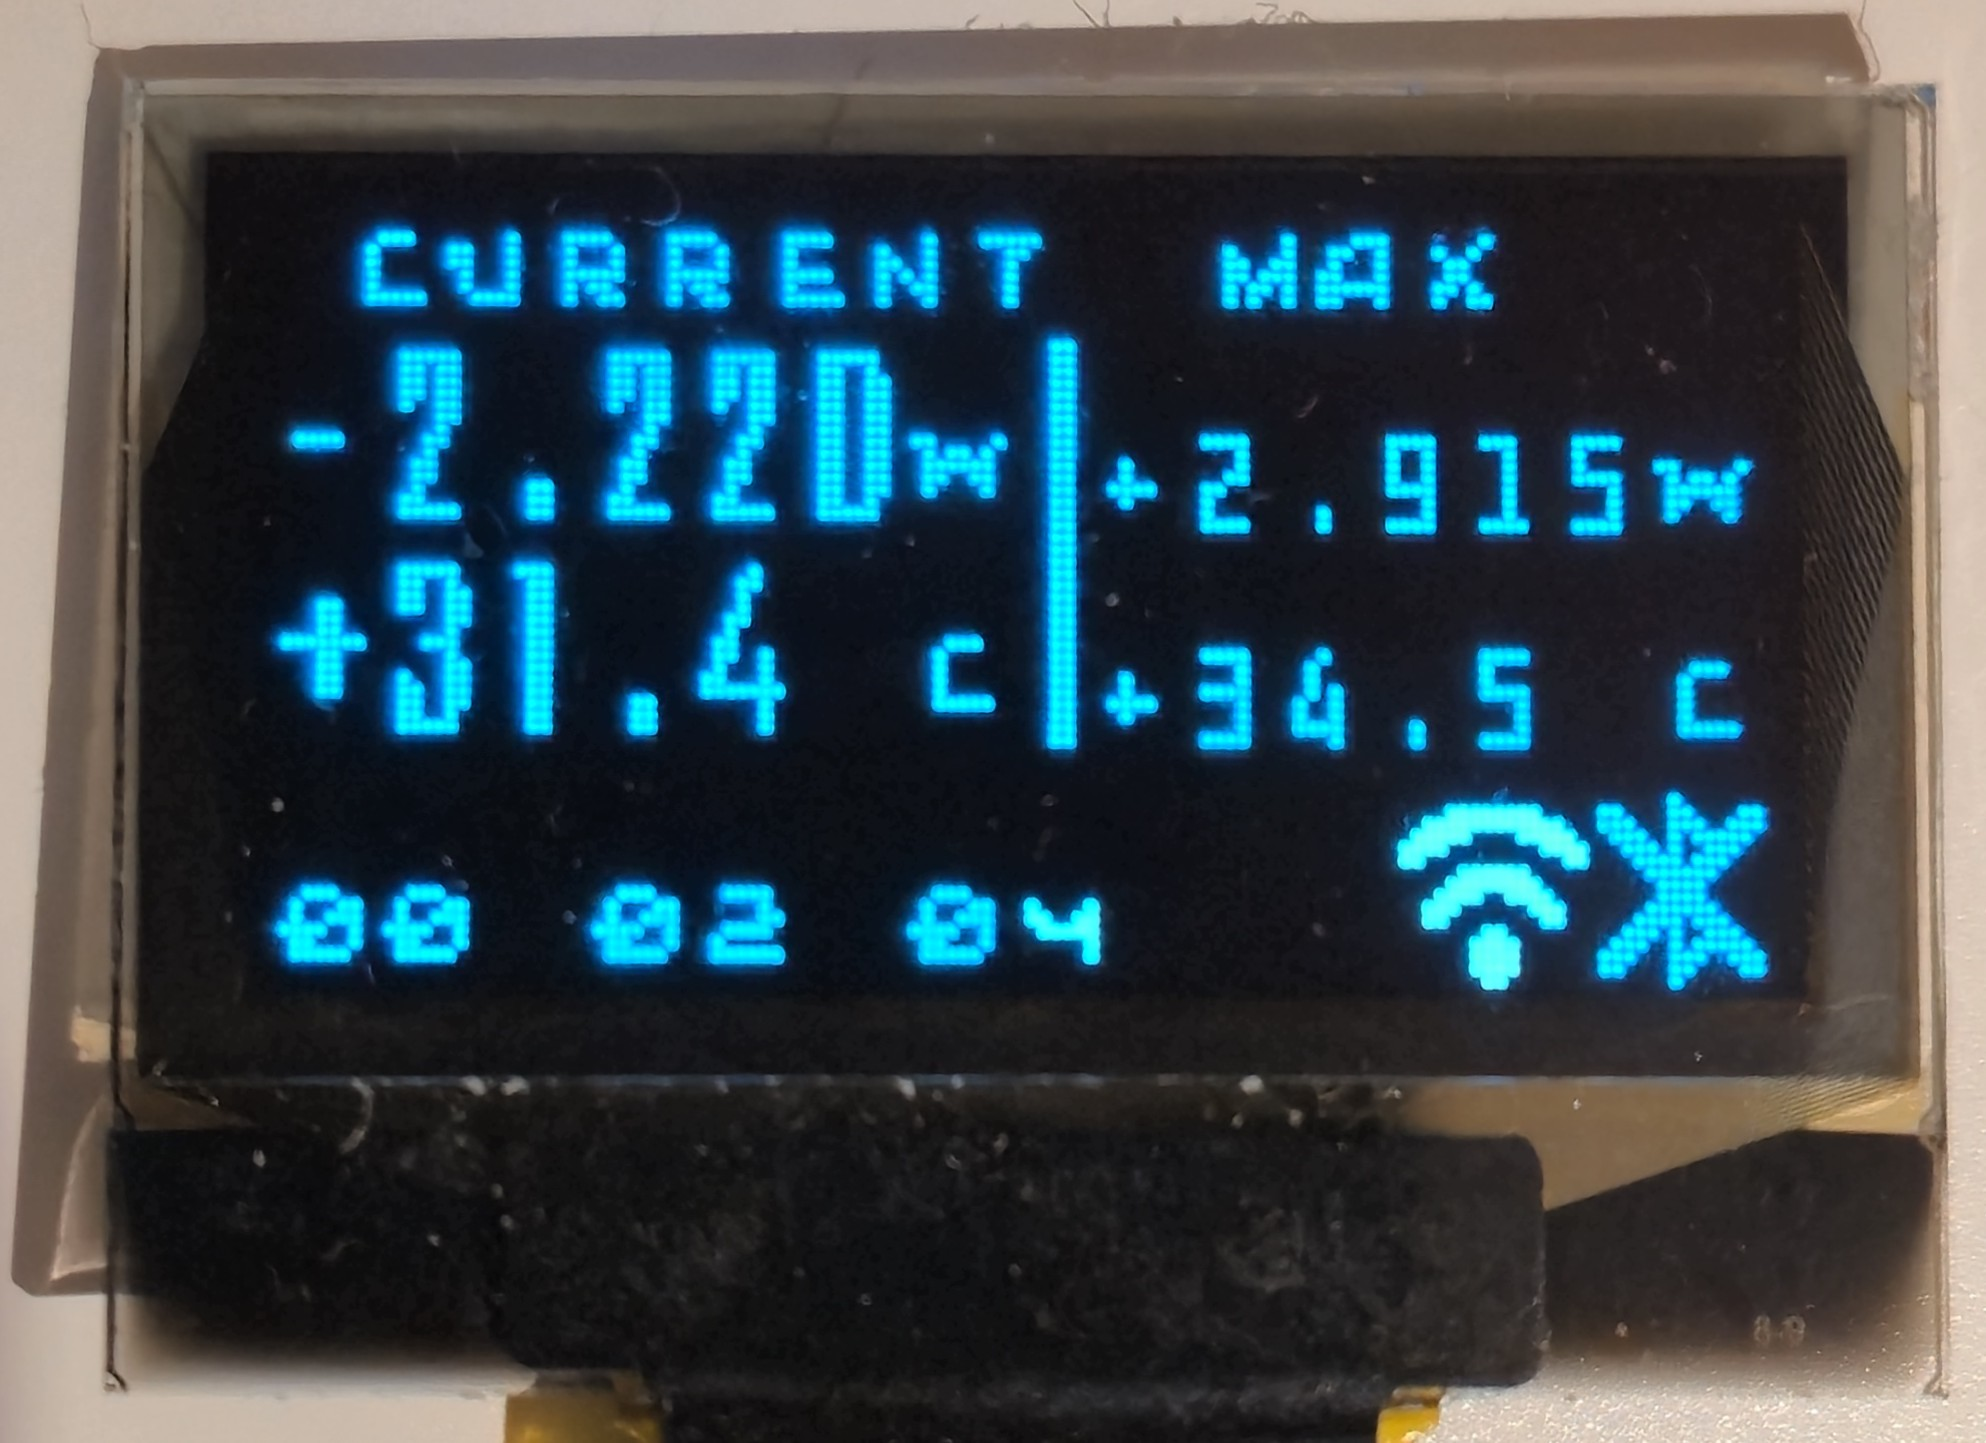
\includegraphics[width=\textwidth]{figures/3_FW_Figures/Page2.jpg}
		\end{minipage}
		
		\captionof{figure}{Live electrical measurement pages shown on the OLED display.}
		\label{fig:display_live_measurements}
		
	\end{center}

	
	\item \textbf{Energy page:} it shows the energy measured during the
	current charge or discharge session and the nominal battery energy configured
	through the BLE application.
	
	\begin{center}
		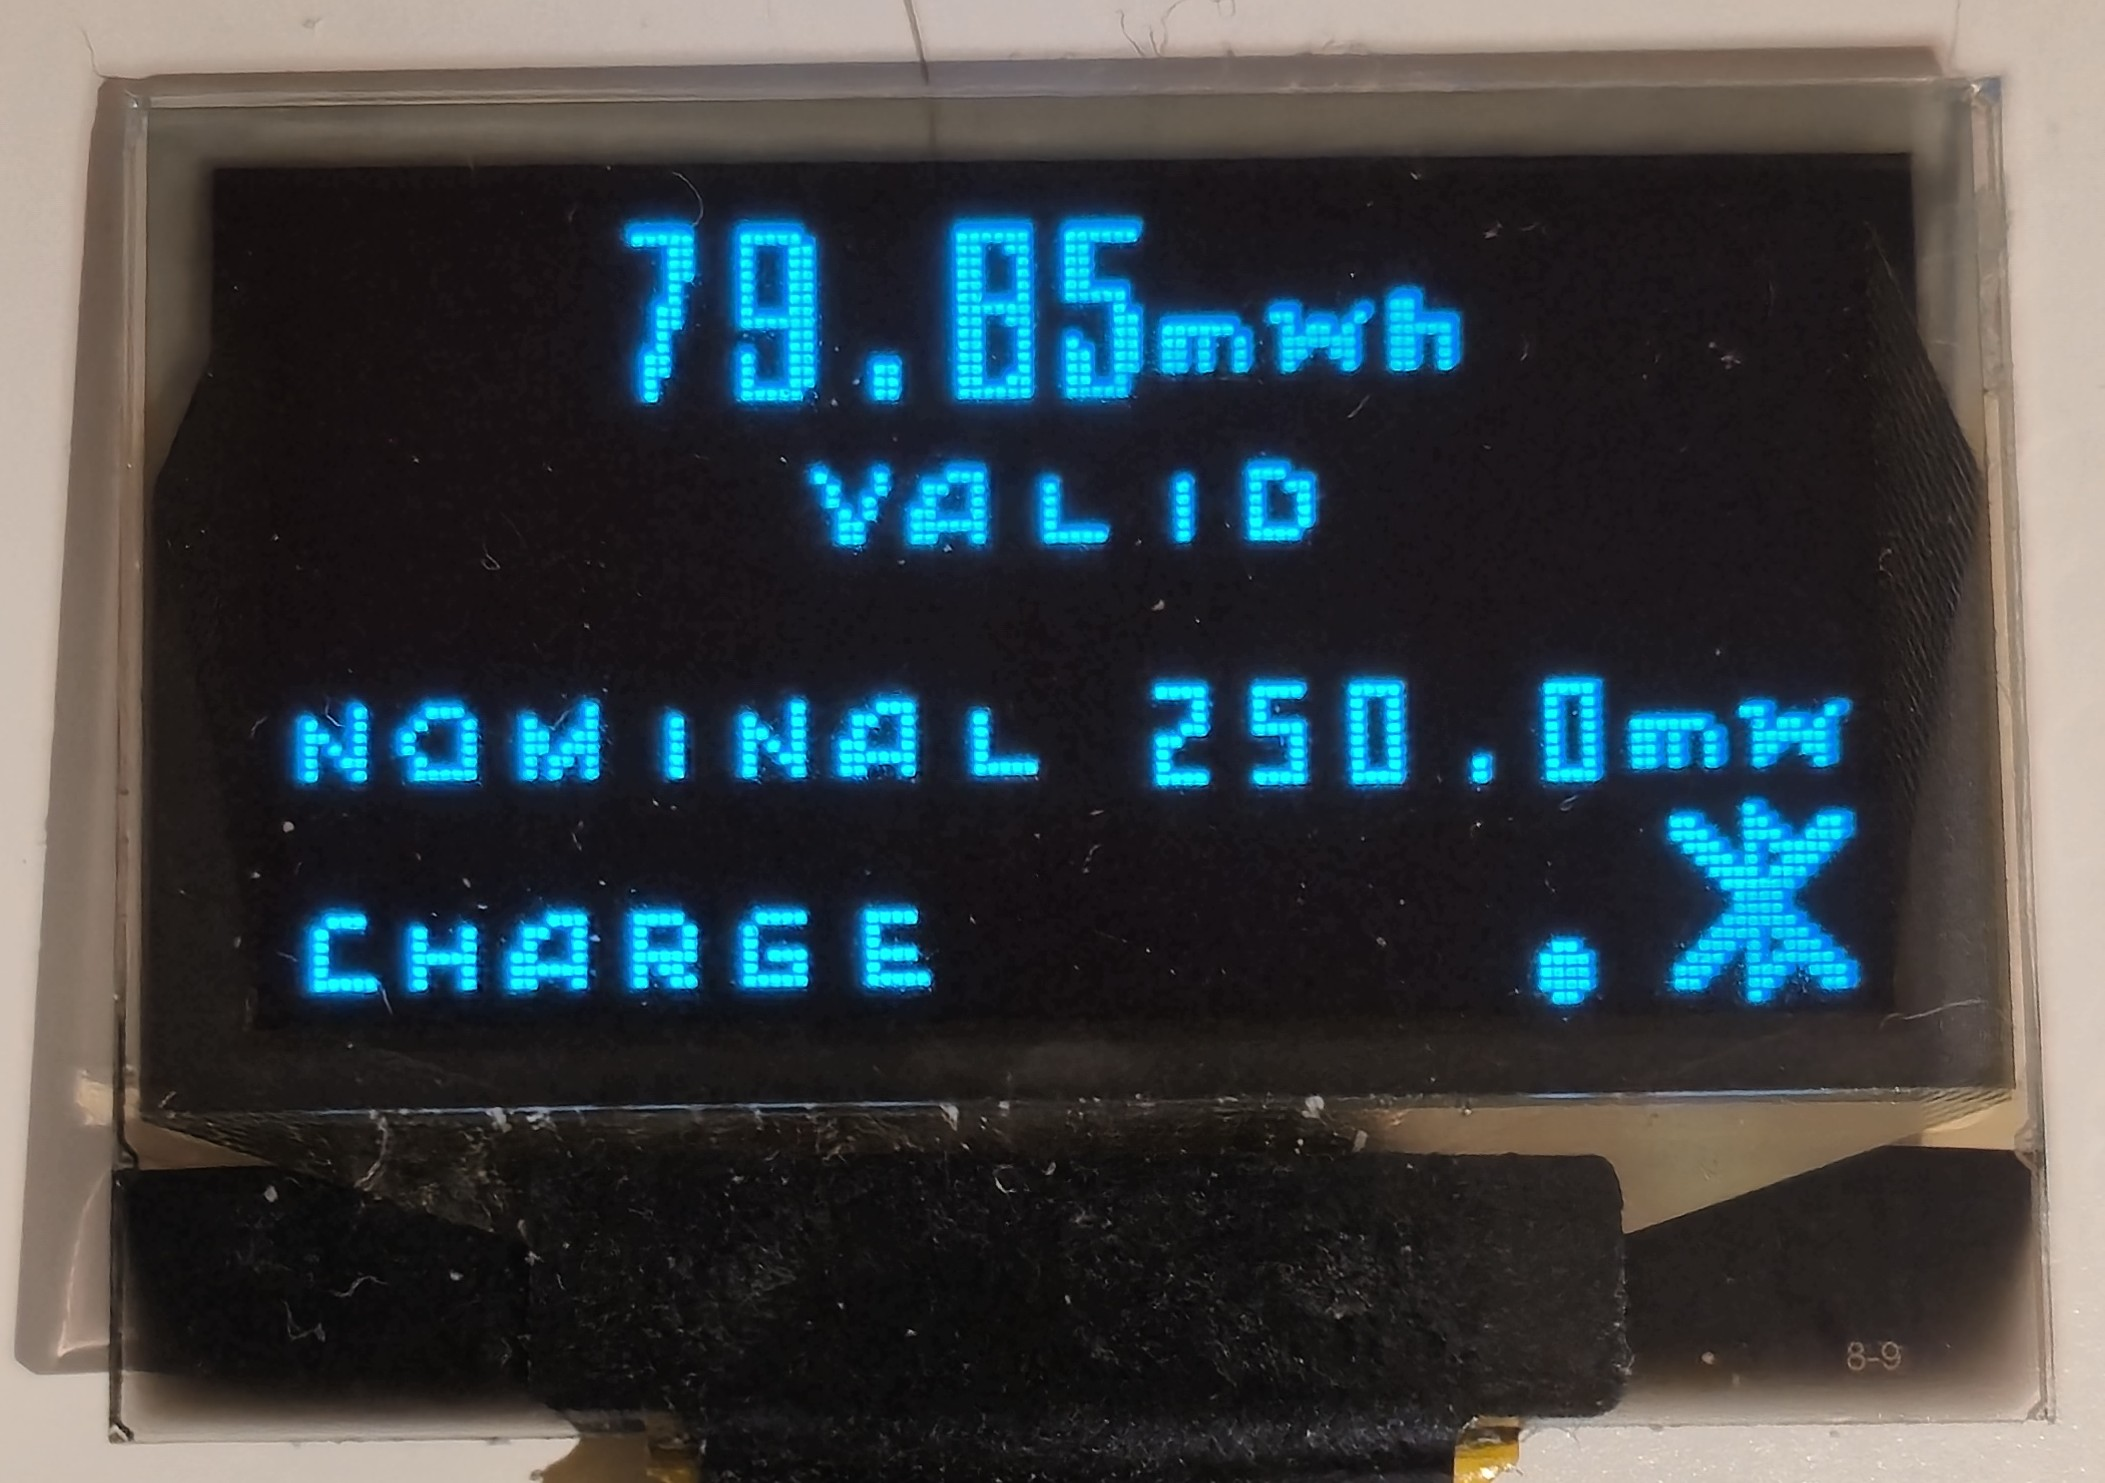
\includegraphics[width=0.30\textwidth]{figures/3_FW_Figures/Page3.jpg}
		\captionof{figure}{Energy page shown on the OLED display.}
		\label{fig:display_energy_page}
	\end{center}
	
	\item \textbf{State of Charge page:} it shows the estimated battery
	State of Charge (SoC), expressed as a percentage.
	
	\begin{center}
		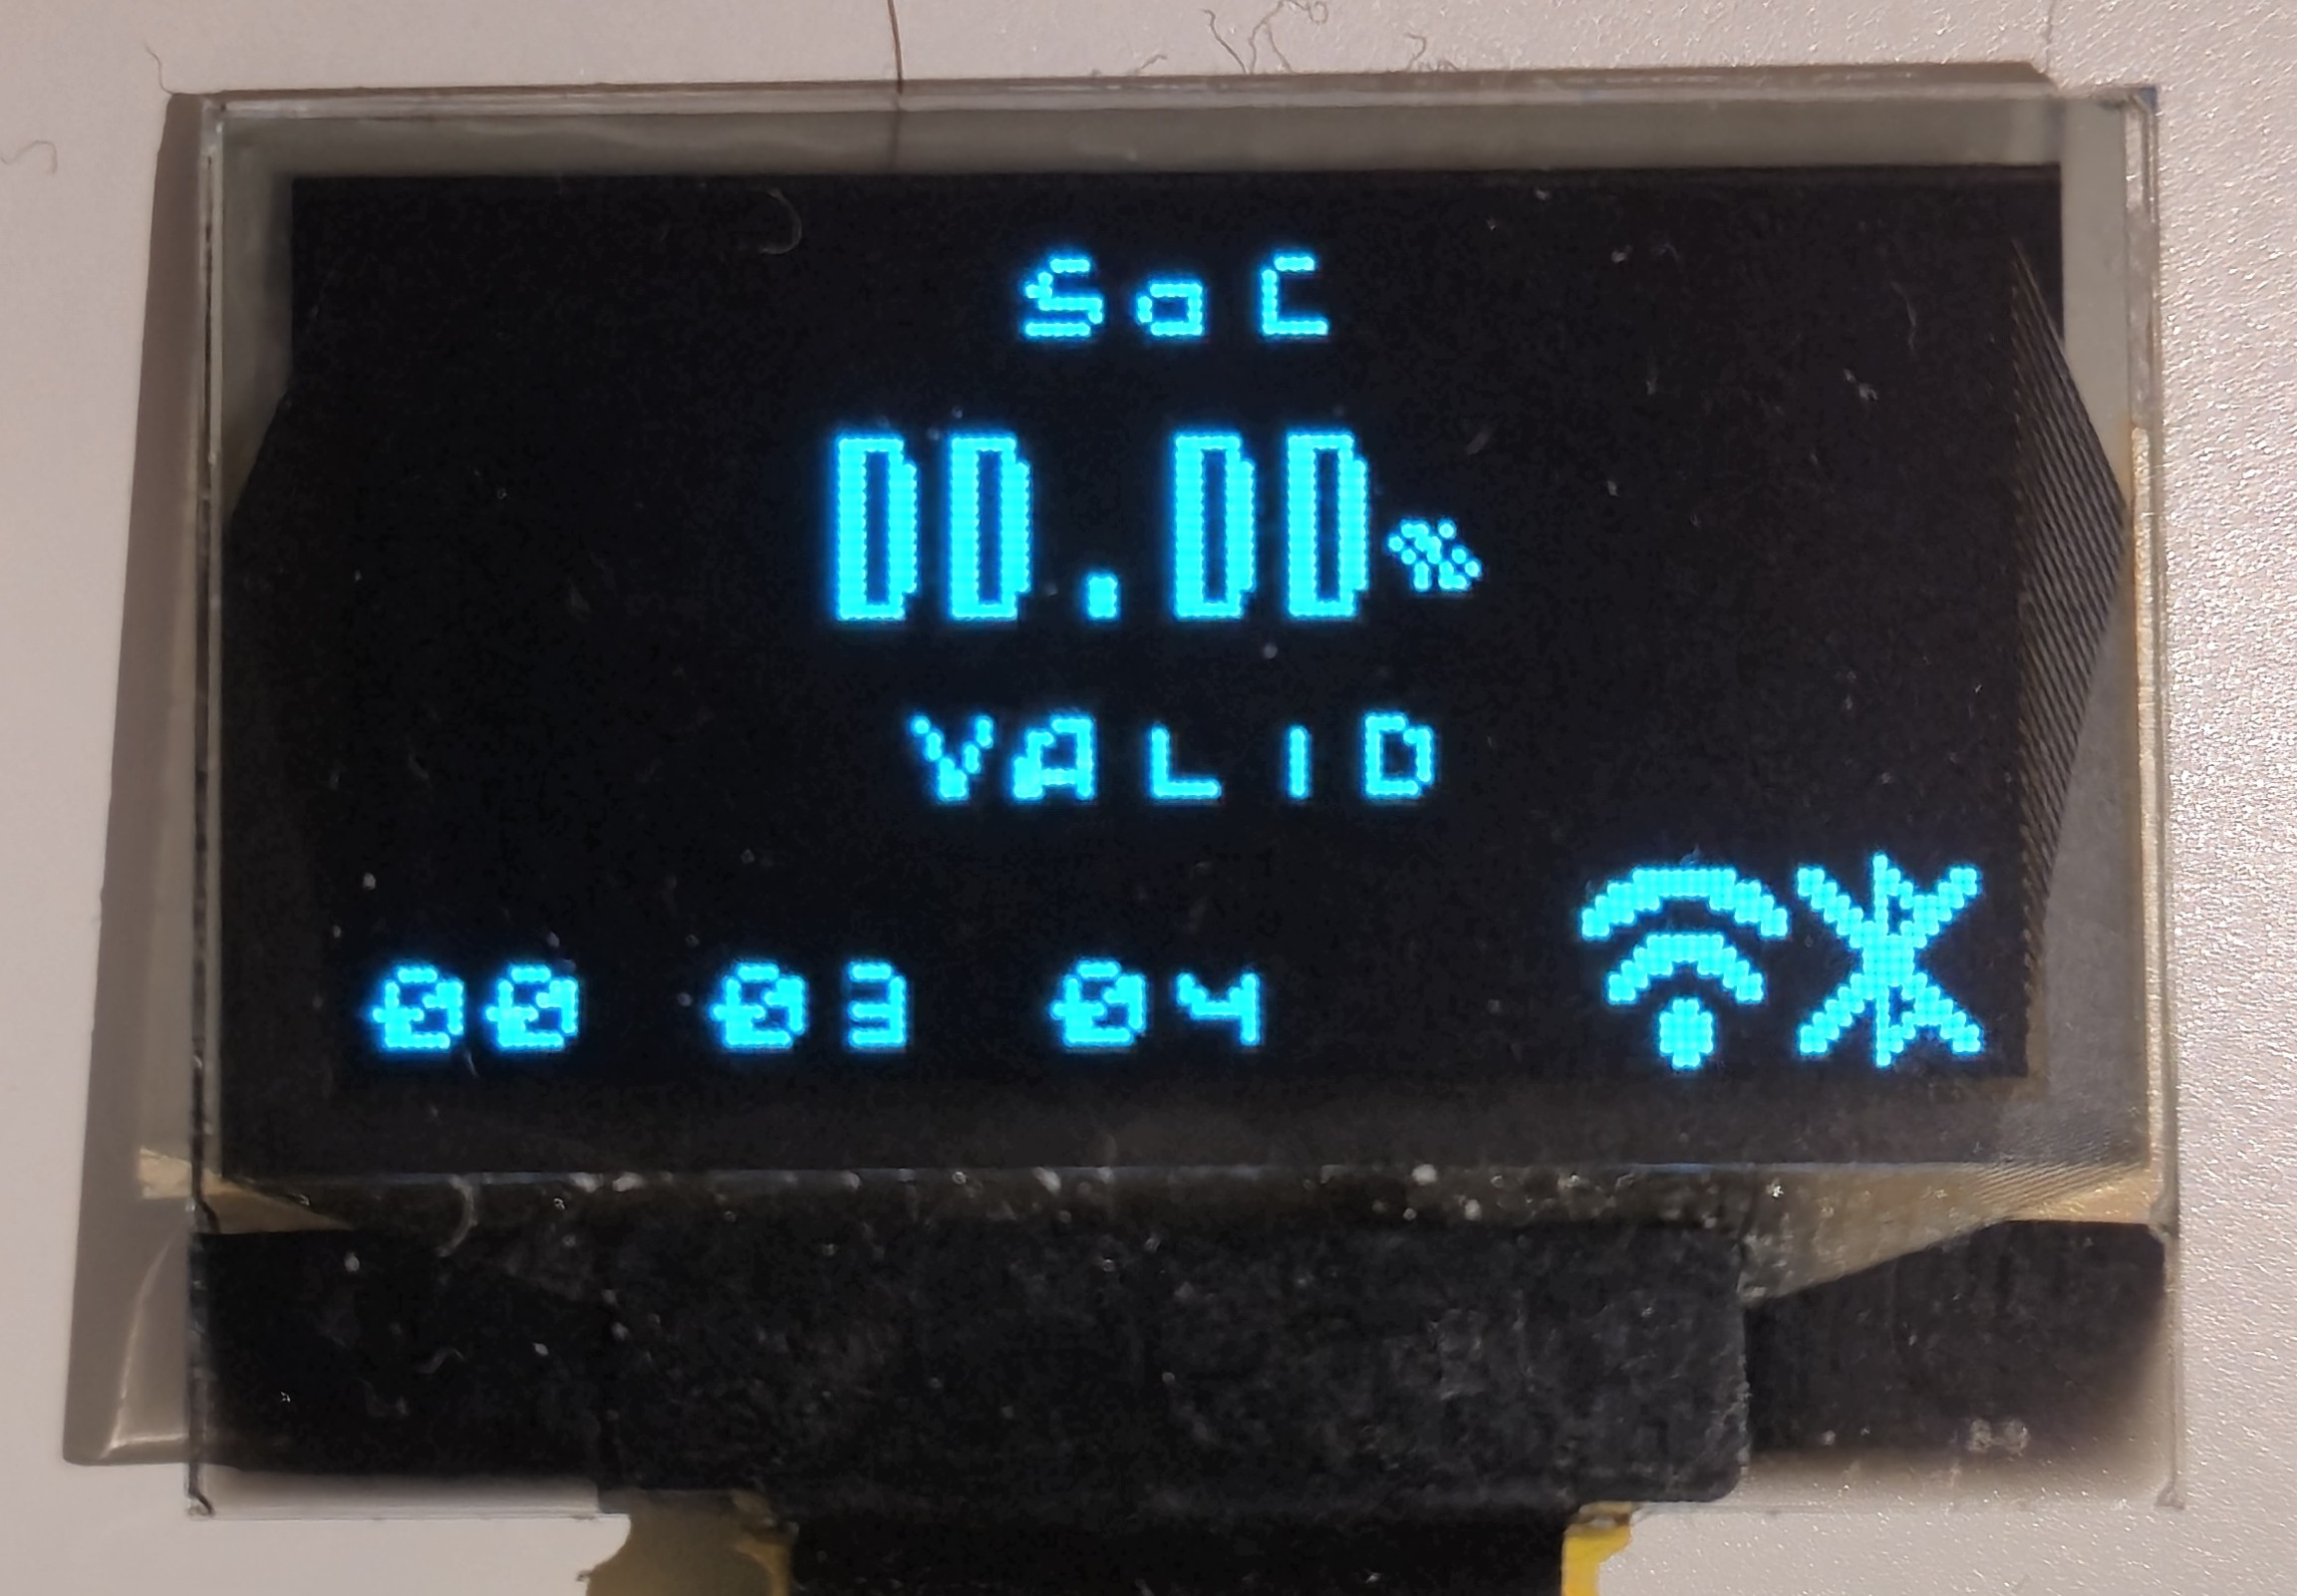
\includegraphics[width=0.30\textwidth]{figures/3_FW_Figures/Page4.jpg}
		\captionof{figure}{State of Charge page shown on the OLED display.}
		\label{fig:display_soc_page}
	\end{center}
	
	\item \textbf{State of Health page:} this page has the same structure as the
	SoC page, but it shows the estimated State of Health (SoH) of the battery.
	
	\begin{center}
		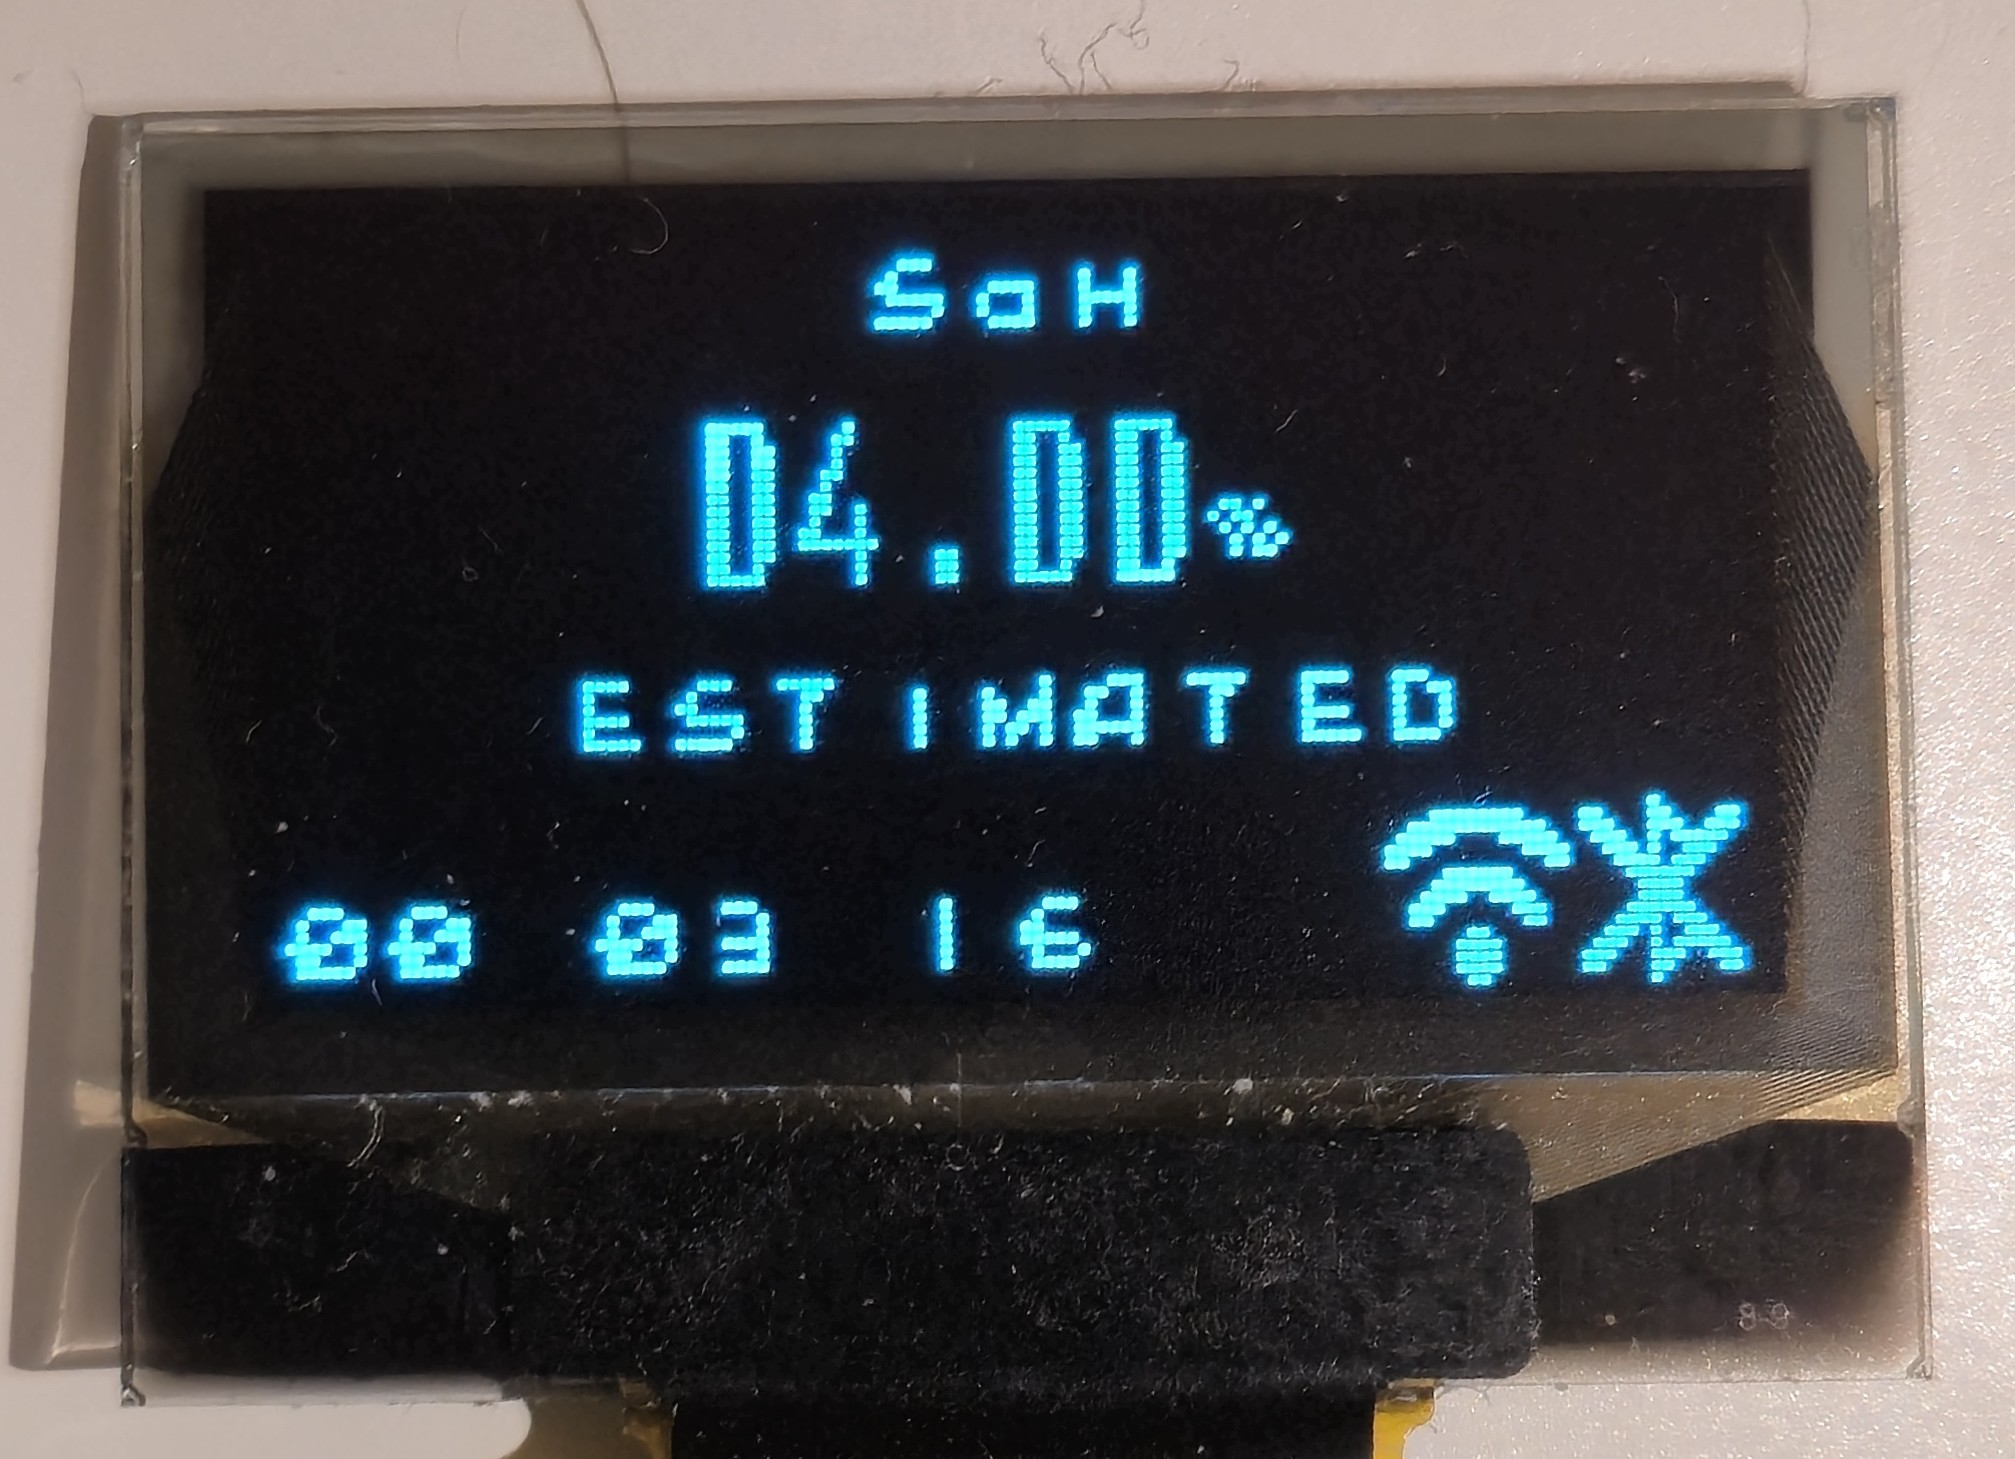
\includegraphics[width=0.30\textwidth]{figures/3_FW_Figures/Page5.jpg}
		\captionof{figure}{State of Health page shown on the OLED display.}
		\label{fig:display_soh_page}
	\end{center}
	
\end{itemize}


All measurements that depend on the previous history of the battery, namely the session energy, SoC and SoH, are accompanied by a tag that shows whether the corresponding value is \texttt{UNKNOWN}, \texttt{ESTIMATED} or \texttt{LEARNED}, as described in Section~\ref{Main_Application_Task}.

All normal pages include a compact footer region used to report secondary status information without affecting the main page content. Depending on the current operating condition, the footer can show either the active session time or the current session state.

The same footer region is also used to display BLE status information. The connection state is represented by a Bluetooth icon, while the link quality is shown through a compact signal indicator derived from the RSSI value provided by the BLE task. In this way, the user can check both the connection state and the approximate BLE signal quality in all avaiabe pages. The icon mapping and RSSI-based signal indication are summarized in Table~\ref{tab:ble_icon_display} and Table~\ref{tab:ble_signal_display}, respectively.

\begin{table}[H]
	\centering
	\small
	\caption{Bluetooth icons used by the OLED interface.}
	\label{tab:ble_icon_display}
	\begin{tabularx}{\textwidth}{
			@{}
			>{\raggedright\arraybackslash}X
			>{\raggedright\arraybackslash}X
			>{\centering\arraybackslash}m{1.6cm}
			@{}
		}
		\toprule
		\textbf{BLE connection state} &
		\textbf{Bluetooth icon} &
		\textbf{Symbol} \\
		\midrule
		
		Disconnected or advertising &
		Crossed Bluetooth icon &
		\tableicon{figures/NO_BLE_16x16.png} \\
		
		Connected &
		Bluetooth icon &
		\tableicon{figures/BLE_16x16.png} \\
		
		\bottomrule
	\end{tabularx}
\end{table}

\begin{table}[H]
	\centering
	\small
	\caption{BLE signal indicator selection based on connection state and RSSI.}
	\label{tab:ble_signal_display}
	\begin{tabularx}{\textwidth}{
			@{}
			>{\raggedright\arraybackslash}X
			>{\raggedright\arraybackslash}X
			>{\centering\arraybackslash}m{1.6cm}
			@{}
		}
		\toprule
		\textbf{BLE / RSSI state} &
		\textbf{Displayed signal indicator} &
		\textbf{Symbol} \\
		\midrule
		
		Idle, not connected and not advertising &
		Hidden &
		-- \\
		
		Advertising &
		Animated search indicator &
		-- \\
		
		Connected, RSSI $< -75$ dBm &
		Hidden &
		-- \\
		
		Connected, $-75 \leq \mathrm{RSSI} < -60$ dBm &
		Low signal indicator &
		\tableicon{figures/BLE_anim2.png} \\
		
		Connected, $-60 \leq \mathrm{RSSI} < -45$ dBm &
		Medium signal indicator &
		\tableicon{figures/BLE_anim3.png} \\
		
		Connected, $\mathrm{RSSI} \geq -45$ dBm &
		Strong signal indicator &
		\tableicon{figures/BLE_anim4.png} \\
		
		\bottomrule
	\end{tabularx}
\end{table}

\paragraph{Warning overlay.}
Safety warnings are not implemented as a separate display page. Instead, when a danger condition is active, the Display task draws a warning banner on top of the currently selected page. This makes the warning visible independently of the page currently selected by the user. The danger state is still computed by the App task, while the Display task only renders the corresponding visual indication.

\begin{center}
	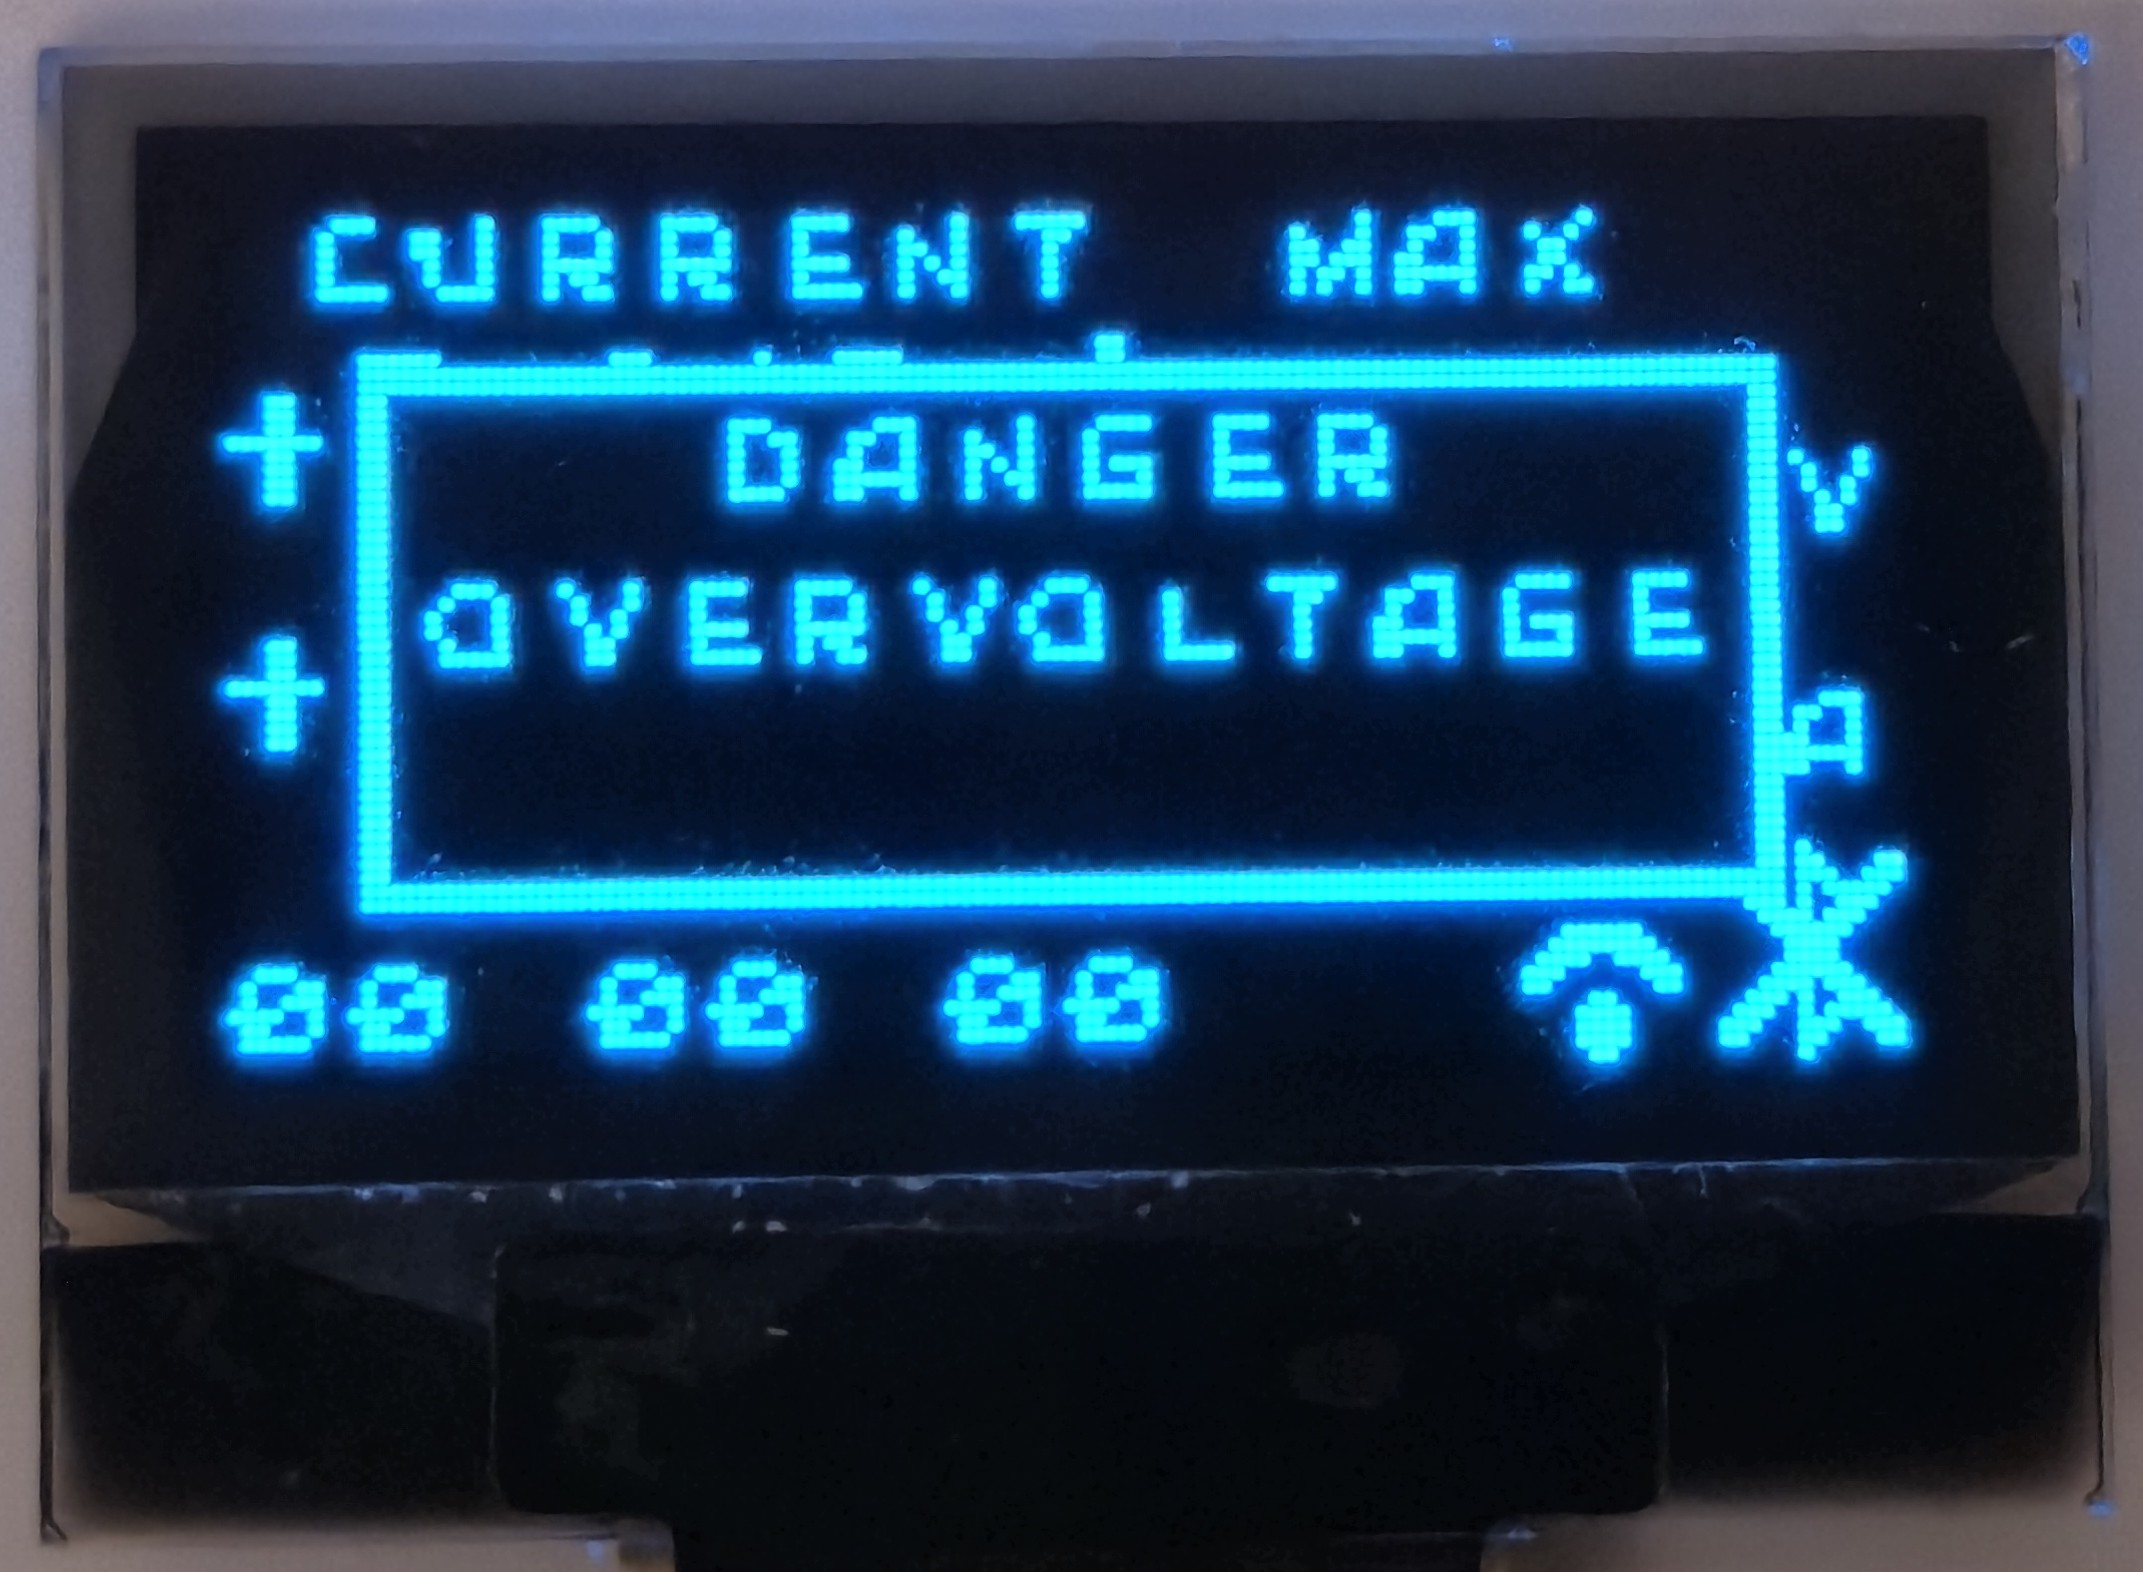
\includegraphics[width=0.30\textwidth]{figures/3_FW_Figures/Page7.jpg}
	\captionof{figure}{Energy page shown on the OLED display.}
	\label{fig:display_danger}
\end{center}

\subsection{Flash Storage Application Task}

The Flash Storage task provides the non-volatile storage backend for the battery estimation state. It is implemented as a separate RTOS task because flash program and erase operations are slower and more restrictive than normal RAM accesses. The App task does not access the flash driver directly; instead, it posts high-level storage requests to the Flash Storage mailbox, while the Flash Storage task performs the required low-level operations.

Although the amount of data to be preserved is small, the firmware uses one available flash page as an append-only log. This avoids treating flash as a directly overwritten variable and reduces the number of page erase operations required during normal operation.

\paragraph{Stored records.}
The flash page is shared by two record classes, selected according to their update rate. Fast checkpoint records are written periodically during active charge or discharge sessions and are used to recover the current session after an unexpected reset. Slow records are written only when long-term battery information changes, such as the configured nominal energy or the last completed cycle energy.

Keeping both record types in the same flash page avoids reserving separate pages for small amounts of data. The available space is instead split according to the expected write rate of each record type, assigning most of the page to frequent checkpoints and a smaller area to slow records.

\begin{table}[H]
	\centering
	\small
	\caption{Flash record types used by the Flash Storage task.}
	\label{tab:flash_record_types}
	\begin{tabularx}{\textwidth}{l l X}
		\toprule
		\textbf{Record type} & \textbf{Size} & \textbf{Stored information} \\
		\midrule
		Fast checkpoint &
		8 bytes &
		Sequence counter, current cycle energy, flags, and CRC. \\
		
		Slow record &
		16 bytes &
		Nominal battery energy, last completed cycle energy, completed cycle count, last completed session state, flags, and CRC. \\
		\bottomrule
	\end{tabularx}
\end{table}

Fast checkpoints allow the firmware to recover the current session energy if the device resets during a charge or discharge cycle. Slow records preserve longer-term information, such as the configured nominal energy and the last learned cycle energy used for SoC and SoH estimation.

\paragraph{Append-only storage and recovery.}
Flash memory cannot be overwritten freely: bits can be programmed from \(1\) to \(0\), but returning them to \(1\) requires erasing the whole flash page. For this reason, each new record is written in the next empty slot of its corresponding area. When the available slots are exhausted, the page is erased and the latest record that must be preserved is written again after the erase.

At startup, the Flash Storage task scans the reserved page to reconstruct the last stored state. Empty records are ignored, while programmed records are decoded and ordered using their sequence counter. The newest valid record is then selected as the current non-volatile state. This allows the firmware to recover the latest stored information without overwriting previous records in place.

\paragraph{Flash page allocation and endurance.}
The reserved flash page has a size of \(B_{page} = 4096\,\mathrm{B}\). The split between fast and slow records is computed from the expected write periods and record sizes:

\begin{itemize}
	\item fast checkpoint period: \(T_f = 30\,\mathrm{s}\);
	\item average slow record period: \(T_s = 3600\,\mathrm{s}\);
	\item fast record size: \(S_f = 8\,\mathrm{B}\);
	\item slow record size: \(S_s = 16\,\mathrm{B}\).
\end{itemize}

The amount of flash reserved for slow records is selected so that the fast and slow areas are consumed at approximately the same rate. The ideal value is then rounded to an integer number of slow records:

\[
B_s^\star =
\frac{B_{page} \cdot T_f \cdot S_s}
{T_f \cdot S_s + T_s \cdot S_f}
=
\frac{4096 \cdot 30 \cdot 16}
{30 \cdot 16 + 3600 \cdot 8}
\approx
67\,\mathrm{B}
\xrightarrow{B_s = 64\,\mathrm{B}}
\left\{
\begin{aligned}
	N_s &= \frac{B_s}{S_s} = \frac{64}{16} = 4 \\
	N_f &= \frac{B_{page} - B_s}{S_f} = \frac{4096 - 64}{8} = 504
\end{aligned}
\right.
\]

The resulting allocation provides \(4\) slow records and \(504\) fast checkpoints in one flash page. With one checkpoint every \(30\,\mathrm{s}\), the fast area covers:

\[
T_{page,f} =
N_f \cdot T_f
=
504 \cdot 30\,\mathrm{s}
=
15120\,\mathrm{s}
\approx
4.2\,\mathrm{h}
\]

A similar calculation can be performed for the slow area, which provides approximately \(4\,\mathrm{h}\) of operation before the slow-record slots are exhausted. Therefore, the two areas are consumed at approximately the same rate.

Therefore, the two areas are consumed at approximately the same rate.

Considering a flash endurance of \(100000\) erase cycles, the theoretical active-session endurance is:

\[
T_{\mathrm{active,max}} =
100000 \cdot T_{page,f}
=
100000 \cdot 504 \cdot 30\,\mathrm{s}
=
1.512 \cdot 10^9\,\mathrm{s}
=
420000\,\mathrm{h}
\approx
47.9\,\mathrm{years}
\]

This value represents the theoretical lifetime during charge or discharge activity. Periods in which WattMate is powered on, but no power is transmitted on the USB bus is not counted in this computation, because in that case no new record is saved on Flash Memory.

\paragraph{Data integrity.}
Each record contains a CRC field. After programming a record, the Flash Storage task reads it back and decodes it again before updating the in-RAM storage state. During startup scanning, records with an invalid CRC are discarded. This prevents partially written or corrupted records from being used as valid battery state.


\subsection{Input Application Task}
\label{sec:input_task}

The Input task manages the physical inputs of WattMate and converts low-level hardware events into application-level events. Its role is intentionally limited: it does not decide the system behavior, but it detects user actions, PAC alert signals, and temperature samples, then immediately notifies the App task.

\paragraph{User button handling.}
The user button is handled through GPIO interrupts and RTOS timers. When an edge is detected, the button interrupt is temporarily disabled and a debounce timer is started. The debounce time is set to \(30\,\mathrm{ms}\). After this interval, the button level is sampled again and the task decides whether a valid press or release occurred.

A second timer is used for long-press detection. If the button remains active for \(800\,\mathrm{ms}\), the Input task posts a long-press event to the App task. Otherwise, when the button is released before the long-press timeout, a normal button-press event is generated. This allows the App task to receive clean user events without directly handling mechanical bouncing or button timing.

\paragraph{PAC alert inputs.}
The PAC1951 alert pins are also managed by the Input task. These pins are configured as interrupt sources and are used to notify the App task when a hardware alert occurs. In this way, configured PAC1951 alert conditions can be forwarded immediately to the App task, without waiting for the next standard I2C communication cycle.

\paragraph{Temperature sampling.}
The NTC temperature measurement is controlled by the Input task through the ADC driver. Sampling is not always active: the App task enables the temperature measuremnets according to the current runtime needs commanded by the App task, for example when the display is showing temperature information or when BLE telemetry is active.

When temperature sampling is enabled, the Input task performs one sample every \(200\,\mathrm{ms}\). For each sample, the task enables the NTC divider, waits \(5\,\mathrm{ms}\) to let the analog node settle, and then performs the ADC conversion. 

The raw ADC value is converted into centi-degrees Celsius using a precomputed NTC lookup table. The table is generated offline from the NTC beta model, using

\[
R_{NTC}(T) =
R_0 e^{B\left(\frac{1}{T_K} - \frac{1}{T_0}\right)}
\]

where \(R_0 = 10\,\mathrm{k\Omega}\), \(T_0 = 298.15\,\mathrm{K}\), and
\(B = 3435\,\mathrm{K}\). Given the hardware NTC circuit, the expected ADC code
for each temperature is computed as

\[
ADC_{LUT}(T) =
ADC_{max}
\frac{V_{DD}}{V_{FS}}
\frac{R_{NTC}(T)}{R_1 + R_{NTC}(T)}.
\]

In the current firmware, the LUT is generated assuming \(V_{DD}=3.3\,\mathrm{V}\). However, the real board supply voltage is provided by the DC/DC converter and can be slightly different from this nominal value. Since the ADC code depends on the voltage applied to the NTC circuit, using the raw ADC value directly would introduce a temperature error whenever the real supply voltage differs from \(3.3\,\mathrm{V}\).

For this reason, before accessing the lookup table, the firmware reads the actual board supply voltage using the internal battery monitor of the MCU and rescales the measured ADC code to the equivalent value that would have been measured with the nominal LUT supply voltage:

\[
ADC_{scaled} =
ADC_{raw}
\frac{V_{DD,LUT}}{V_{DD,meas}}.
\]

The lookup table is then searched using \(ADC_{scaled}\), not the uncorrected raw ADC value. Since the LUT contains discrete points, the final temperature is obtained by linear interpolation between the two adjacent table entries. If

\[
ADC_i \geq ADC_{scaled} \geq ADC_{i+1},
\]

the temperature is computed as

\[
T =
T_i +
\frac{ADC_i - ADC_{scaled}}{ADC_i - ADC_{i+1}}
\left(T_{i+1} - T_i\right).
\]

The resulting value is stored in centi-degrees Celsius. This approach avoids evaluating the full NTC equation at runtime, while still compensating for supply-voltage variations of the board.



\subsection{PAC Application Task}
\label{PAC_Application_Task}

The PAC1951 Application task manages the interface between WattMate and the PAC1951 power monitor. Its role is to configure the sensor, select the appropriate sampling profile, control when I2C measurement reads are performed, and publish electrical measurement snapshots to the App task.

The task is separated from the main App task because the PAC1951 is not only a measurement device. It also provides hardware alert outputs, internal sampling configuration, programmable thresholds, and an energy accumulator. Keeping these details inside the PAC task allows the App task to request high-level sensor actions without directly handling the PAC1951 driver configuration.

The App task interacts with the PAC task through high-level commands posted to its RTOS mailbox. These commands do not directly access the PAC1951 driver; they only request sensor-level actions. The detailed execution is handled internally by the PAC task. The main command categories are summarized in Table~\ref{tab:pac_task_commands}.

\begin{table}[H]
	\centering
	\small
	\caption{Main command categories handled by the PAC task.}
	\label{tab:pac_task_commands}
	\begin{tabularx}{\textwidth}{lX}
		\toprule
		\textbf{Command category} & \textbf{Purpose} \\
		\midrule
		Profile control & Switch the PAC1951 between idle and normal sampling profiles. \\
		Measurement stream control & Enable or disable periodic I2C reads from the PAC1951. \\
		Accumulator read control & Enable or disable PAC1951 accumulator reads. \\
		\bottomrule
	\end{tabularx}
\end{table}

\paragraph{PAC1951 configuration.}
The PAC1951 is configured as the main electrical measurement device of WattMate. The bus-voltage measurement is configured as unipolar, while the sense-current measurement is configured as bipolar, allowing the firmware to represent both charge and discharge current directions.

The accumulator is configured in power accumulation mode. This allows the accumulated quantity to be directly converted into energy over time. When energy measurement is enabled, the PAC task reads the accumulator contribution, adds it to the current session energy counter, and publishes the updated energy value together with the live electrical snapshot.

\begin{table}[H]
	\centering
	\small
	\caption{Main PAC1951 measurement configuration.}
	\label{tab:pac_measurement_configuration}
	\begin{tabularx}{\textwidth}{lX}
		\toprule
		\textbf{Measurement} & \textbf{PAC1951 configuration} \\
		\midrule
		Bus voltage & Channel 1 bus-voltage measurement, configured as unipolar. \\
		Sense current & Channel 1 sense-voltage measurement, configured as bipolar and converted using a \(10\,\mathrm{m\Omega}\) sense resistor. \\
		Power & Computed by the PAC1951 from bus voltage and sense current. \\
		Energy & Obtained by configuring the PAC1951 accumulator in power accumulation mode. \\
		\bottomrule
	\end{tabularx}
\end{table}

\paragraph{Sampling profiles.}
The PAC task defines two sampling profiles. Each profile represents a complete PAC1951 operating configuration, including sampling mode, alert routing, thresholds, and alert sample counts. The profiles used by WattMate are summarized in Table~\ref{tab:pac_sampling_profiles}.

\begin{table}[H]
	\centering
	\small
	\caption{PAC1951 sampling profiles used by WattMate.}
	\label{tab:pac_sampling_profiles}
	\begin{tabularx}{\textwidth}{lXX}
		\toprule
		\textbf{Parameter} & \textbf{Idle profile} & \textbf{Normal profile} \\
		\midrule
		Sampling mode &
		\(8\) samples/s, adaptive accumulation mode &
		\(64\) samples/s, adaptive accumulation mode \\
		
		Main purpose &
		Bus activity detection with reduced sampling activity &
		Active charge/discharge measurement and safety supervision \\
		
		\texttt{ALERT1} routing &
		Electrical safety detection &
		Electrical safety detection \\
		
		\texttt{ALERT2} routing &
		Over-power event used as wake-up source &
		Accumulator-fullness indication \\
		
		Over-power threshold &
		\(50\,\mathrm{mW}\) &
		Not used for wake-up \\
		
		Safety thresholds &
		\(30000\,\mathrm{mV}\) overvoltage,
		\(5000\,\mathrm{mA}\) overcurrent &
		\(30000\,\mathrm{mV}\) overvoltage,
		\(5000\,\mathrm{mA}\) overcurrent \\
		
		Safety alert sample count &
		\(4\) samples &
		\(4\) samples \\
		
		Wake-up alert sample count &
		\(1\) sample &
		Not used \\
		\bottomrule
	\end{tabularx}
\end{table}

The idle profile is used when no active charge or discharge session is present. In this mode, the PAC1951 is not shut down completely, but continues to monitor the power bus at a reduced sampling rate. This allows the MCU to remain in a low-power state while the PAC1951 autonomously detects relevant bus activity.

This approach avoids periodic one-shot measurements initiated by the MCU. Instead, \texttt{ALERT2} is configured as a wake-up source when the absolute bus power exceeds the session start threshold, equal to \(50\,\mathrm{mW}\). Safety supervision remains active through \texttt{ALERT1}, so overvoltage and overcurrent conditions can still be reported while the system is idle.

The normal profile is used during active charge or discharge sessions. In this mode, the PAC1951 operates at a higher sampling rate to support energy accumulation and real-time supervision. \texttt{ALERT1} remains assigned to electrical safety events, while \texttt{ALERT2} is reconfigured as an accumulator-fullness indication, allowing the firmware to read accumulated measurements when new data are available.

\paragraph{Measurement stream.}
The PAC1951 sampling profile and the MCU measurement stream are intentionally kept separate. The sampling profile defines how the sensor operates internally, while the measurement stream defines whether the MCU periodically reads the latest values through I2C.

When the stream is requested, the PAC task performs an immediate read and then uses an RTOS clock to schedule the following reads according to the active PAC sampling mode. When the stream is released, the clock is stopped and no periodic I2C transactions are performed, even if the PAC1951 remains configured and active.

This separation supports power management. The PAC1951 can continue monitoring the bus with the selected profile, while the MCU avoids unnecessary I2C transactions whenever live measurements are not required by the App task, the display, or the BLE interface.


\subsection{WattMate BLE Application Task}

The WattMate BLE Application task manages the wireless interface of WattMate. Its role is to isolate the BLE stack, the GATT service, advertising, connection events and notification timing from the rest of the firmware. The App task does not call the BLE stack directly; instead, it interacts with the BLE task through high-level commands.

This separation is useful because BLE communication has its own asynchronous execution model. Connection events, characteristic writes, notification availability and RSSI updates are generated by the BLE stack, while the rest of the firmware only needs to know whether the device is connected, whether the mobile application requested streaming, and when BLE data must be published.

\begin{table}[H]
	\centering
	\small
	\caption{Main command categories handled by the WattMate BLE task.}
	\label{tab:ble_task_commands}
	\begin{tabularx}{\textwidth}{lX}
		\toprule
		\textbf{Command category} & \textbf{Purpose} \\
		\midrule
		Advertising control 		& Start or stop BLE advertising and select the advertising profile. \\
		Stream control 				& Enable or disable periodic BLE notifications. \\
		Connection configuration	& Configure BLE transmission power and connection timing parameters. \\
		GATT event handling			& Process characteristic writes and notify the App task when the mobile application changes a setting. \\
		RSSI monitoring				& Periodically read the connection RSSI and make it available to the App and Display tasks. \\
		\bottomrule
	\end{tabularx}
\end{table}

\paragraph{GATT interface handling.} The BLE task registers and manages the custom GATT service specified in Section~\ref{sec:wattmate_custom_gatt_service} and summarized in Table~\ref{tab:wattmate_gatt_characteristics}. It handles characteristic writes, notification configuration changes, and notification requests, but it does not define the application meaning of the received commands by itself. For example, a write to the Control characteristic, whose payload is specified in Table~\ref{tab:wattmate_control_payload}, is converted into an application event, while the App task decides how the system state must change.

\paragraph{Advertising and connection state.}
The BLE task controls when WattMate is discoverable and selects the active advertising profile according to the current application state. 
The externally visible advertising payload and timing values are reported in Section~\ref{sec:wattmate_advertising_data}, Table~\ref{tab:wattmate_advertising_profiles}, and Figure~\ref{fig:wattmate_advertising_timing}.

When a central device connects, the BLE task updates its internal connection state and notifies the App task. 
When the connection is lost, the stream is stopped, the RSSI value is invalidated, and the App task is informed so that the system can return to the appropriate advertising state.

\paragraph{Telemetry streaming.}
BLE notifications are sent only when a connection is active, the mobile application has enabled the required notification descriptors, and the telemetry stream has been enabled. 
The externally visible notification timing is reported in Section~\ref{sec:wattmate_streaming_timing} and Figure~\ref{fig:wattmate_streaming_timing}.

At each stream update, the BLE task reads the latest application snapshot and packs it into the corresponding GATT payloads. 
The BLE task therefore does not perform measurement acquisition or battery estimation itself; it only publishes the most recent state produced by the App task.

\paragraph{RSSI monitoring.}
While connected, the BLE task periodically requests the RSSI value from the BLE stack. The value is updated every \(1000\,\mathrm{ms}\) and passed to the App state. The Display task can then read this state directly and show the BLE signal quality using the compact signal indicator described in the Display task section.






\section{Additional Firmware Design Aspects}
\subsection{Driver Layer}

The firmware uses two different kinds of drivers. Standard MCU peripherals, such as GPIO, ADC, I2C, Flash and RTOS-related services, are accessed through the Texas Instruments driver layer. These drivers were not modified by the project; they were only configured and used by the application tasks.

The project-specific driver work is instead concentrated on the external devices used by WattMate, especially the PAC1951 power monitor and the SSD1306 OLED controller.

\paragraph{PAC1951 driver.}
The PAC1951 driver was developed specifically for this project, since no suitable open-source C driver was available for the required use case. The driver is kept as an independent module and has also been placed under version control, so that it can be reused or tested separately from the WattMate application logic.

The goal of this driver is to hide the register-level interface of the PAC1951 behind higher-level functions. In particular, the driver provides APIs to:

\begin{itemize}
	\item initialize the device and verify that the expected PAC1951 part is present;
	\item configure the active measurement channel;
	\item select voltage and current measurement ranges;
	\item configure bipolar or unipolar measurements;
	\item configure the internal accumulator mode;
	\item select and route alert sources to the physical alert pins;
	\item program alert thresholds and alert sample counts;
	\item read converted voltage, current, power and accumulated energy values.
\end{itemize}

This separation keeps the PAC Application task independent from the raw register map of the sensor. The PAC task decides when the sensor must be configured, which sampling profile must be active, and when a measurement must be read. The driver, instead, is responsible for translating those requests into the correct PAC1951 register operations and physical-unit conversions.

This boundary also makes the firmware easier to maintain. For example, changing the register sequence needed to configure an alert source affects only the driver implementation, while the PAC task can keep using the same high-level API.

\paragraph{SSD1306 display driver.}
The SSD1306 display driver was adapted from existing C implementations and then extended for the needs of WattMate. The driver owns the local display framebuffer and exposes simple drawing primitives, such as pixels, lines, rectangles, bitmaps and strings.

The Display task uses these primitives to build the actual user interface pages. Therefore, the driver remains responsible only for low-level OLED operations, while the Display task owns the UI state machine, page layout, brightness policy, animations and warning overlays.

For the \(128 \times 64\) monochrome OLED used in WattMate, the framebuffer size
is

\[
B_{\mathrm{fb}} =
128 \cdot \frac{64}{8}
=
1024\,\mathrm{B}.
\]

Although this consumes a relevant amount of SRAM, it simplifies the rendering model: each page is first composed in RAM and then transferred to the OLED controller through I2C. This avoids mixing UI layout code with low-level display transfer details.


\subsection{Memory Constraints}

The firmware runs on a device with limited RAM, while also using the BLE stack, the RTOS kernel, several application tasks and a full display framebuffer. For this reason, memory usage was considered during the firmware design instead of being treated only as a final optimization step. Table~\ref{tab:firmware_memory_overview} summarizes the main memory occupation reported by the linker map.

\begin{table}[H]
	\centering
	\small
	\caption{Firmware memory usage from the linker map.}
	\label{tab:firmware_memory_overview}
	\begin{tabularx}{\textwidth}{l r r X}
		\toprule
		\textbf{Memory region} & \textbf{Total} & \textbf{Used} & \textbf{Comment} \\
		\midrule
		Main Flash &
		\(0x1F000 = 126976\,\mathrm{B}\) &
		\(0x15D89 = 89481\,\mathrm{B}\) &
		Code and constant data. Flash is not the limiting resource in the current build. \\
		
		User Flash page &
		\(0x1000 = 4096\,\mathrm{B}\) &
		\(0x1000 = 4096\,\mathrm{B}\) &
		Reserved Flash page used by the firmware for persistent battery records. Completely used to distribute Flash wear\\
		
		SRAM &
		\(0x4400 = 17408\,\mathrm{B}\) &
		\(0x30E4 = 12516\,\mathrm{B}\) &
		Runtime memory used by stacks, buffers, RTOS objects, BLE structures and global state. \\
		\bottomrule
	\end{tabularx}
\end{table}

The most restrictive memory region is SRAM. The current build leaves

\[
17408 - 12516 = 4892\,\mathrm{B}
\]

of statically free SRAM. This remaining space is important because the BLE stack
and ICall layer also require heap memory at runtime for BLE messages, GATT
operations and asynchronous stack events.

A significant part of the SRAM usage is due only to task stacks and the SSD1306
framebuffer. The main statically allocated stack areas are listed in
Table~\ref{tab:firmware_stack_allocation}.

\begin{table}[H]
	\centering
	\small
	\caption{Main statically allocated stack areas.}
	\label{tab:firmware_stack_allocation}
	\begin{tabularx}{\textwidth}{l r X}
		\toprule
		\textbf{Stack area} & \textbf{Size} & \textbf{Reason} \\
		\midrule
		App task & \(768\,\mathrm{B}\) & Main application state machine and battery estimation logic. \\
		Display task & \(768\,\mathrm{B}\) & UI rendering and SSD1306 driver calls. \\
		WattMate BLE task & \(768\,\mathrm{B}\) & BLE stack event handling and GATT notification logic. \\
		Flash Storage task & \(512\,\mathrm{B}\) & Flash record encoding, validation and program/erase requests. \\
		Input task & \(512\,\mathrm{B}\) & Button timing, PAC alerts and ADC sampling. \\
		PAC task & \(512\,\mathrm{B}\) & PAC1951 configuration and I2C measurement reads. \\
		ICall stack task & \(512\,\mathrm{B}\) & BLE stack interface task. \\
		System stack & \(1024\,\mathrm{B}\) & Interrupts and system-level execution. \\
		\bottomrule
	\end{tabularx}
\end{table}

The total amount of RAM reserved only for these stack areas is

\[
B_{\mathrm{stacks}} =
3 \cdot 768 +
4 \cdot 512 +
512 +
1024
=
5888\,\mathrm{B}.
\]

The SSD1306 display driver also requires a full local framebuffer. For a
\(128 \times 64\) monochrome display, this buffer requires

\[
B_{\mathrm{fb}} =
128 \cdot \frac{64}{8}
=
1024\,\mathrm{B}.
\]

Therefore, stacks and display framebuffer alone reserve

\[
B_{\mathrm{stacks+fb}} =
5888 + 1024
=
6912\,\mathrm{B}.
\]

This is already a large fraction of the available SRAM, before considering task objects, mailboxes, clocks, BLE data structures and the runtime heap. For this reason, the number of application tasks was kept limited to the subsystems that really need independent timing or ownership: App, Display, Input, PAC, Flash Storage and BLE.

The stack size of each task was also selected according to its actual role. Tasks with relatively simple event processing, such as Input, PAC and Flash Storage, use smaller stacks. Tasks that execute more complex logic or interact with larger libraries, such as App, Display and BLE, use larger stacks. This avoids assigning the same conservative stack size to every task, which would waste RAM quickly on this device.

The firmware also avoids large dynamic allocations in the application layer. Most application data structures are statically allocated, while dynamic allocation is mainly left to the BLE/ICall layer, where it is required by the stack event model. This makes RAM usage more predictable and reduces the risk of heap fragmentation caused by application code.


